\documentclass[sigconf]{acmart}
\usepackage[utf8]{inputenc}
\usepackage[T1]{fontenc}
\usepackage{graphicx}
\usepackage{booktabs}
\usepackage{comment}
\usepackage{amsmath,amssymb}
\usepackage{siunitx}
\usepackage{microtype}

\usepackage{xcolor}
\usepackage{url}
%\usepackage[hidelinks]{hyperref}

\newcommand{\ie}{i.e., }
\newcommand{\eg}{e.g., }
\newcommand{\etc}{etc.}

\title{GLOW: Accelerating Geometric Multigrid Layers on Cerebras Wafer-Scale Engine}
\author{Anonymous Submission}



\begin{abstract}
This paper describes the mapping of Geometric Multigrid (GMG) onto the Cerebras Wafer Scale Engine (WSE-3).  The WSE wafer integrates almost a million cores along with a low-latency 2D mesh network, providing unprecedented on-chip bandwidth and fine-grained communication. Although the architecture is predominantly used for deep learning, we explore the suitability of WSE for accelerating GMG. %, focusing on the WSE-3 generation.   Multigrid (MG) methods 
GMG solves sparse linear systems efficiently by recursively coarsening the grid, %making them both fast and highly scalable for scientific computing.  
which leads to more rapid convergence with less computation.
%The underlying GMG operators include stencil application, restriction, prolongation, smoothing, and a bottom solver.  
As compared to prior implementations of stencils on WSE, this demonstration highlights the challenges of mapping a layered algorithm -- and the full set of operators -- onto a dataflow architecture.  We use this implementation as a foundation to discuss the potential for a variety of data and computation mappings of GMG to WSE, and performance compared to the HPGMG benchmark on an NVIDIA H200 GPU.  Across different GMG configurations and problem sizes, we observe a speedup of up to 25$\times$ as compared to a single H200 node.  
\end{abstract}

\begin{document}
\keywords{Spatial dataflow architecture, Geometric multigrid}
\maketitle

\section{Introduction}
%\textbf{Problem motivation}
Geometric multigrid (GMG) is an important family of algorithms used by computational scientists to accelerate the convergence of iterative solvers for linear systems of the form $Ax=b$.  It is a multigrid because computation is mapped to a hierarchy of coarser grid levels.  As shown in Figure~\ref{fig 1:V-cycle in GMG}, the underlying GMG operators include stencil application, residual, restriction, interpolation, smooth, and a direct (bottom) solver. In such a formulation, the floating-point computation in GMG is dwarfed by the overhead of data movement (during stencil application and across levels), making managing the memory hierarchy and cross-processor communication critical to achieving high performance.    
%Solving large systems of linear equations lies at the core of numerous scientific and engineering applications, including computational fluid dynamics (CFD), climate and weather modeling, etc. These physical problems are typically formulated as non-linear Partial Differential Equations (PDEs), which upon discretization using finite differences, volumes, or elements to produce large, sparse linear systems of the form $Ax=b$. Efficiently solving these systems is critical for large-scale numerical simulation. Among the broad landscape of linear solvers—such as direct methods, classical iterative solvers, and Krylov subspace solvers, Multigrid (MG) methods stand out because they achieve optimal O(N) computational complexity and scalable across thousands of nodes on modern HPC systems. \textcolor{red}{This first paragraph is overly broad.  I think you should just motivate multigrid without all the other things.  Then add references that are focused on what you discuss.}
%\textbf{Hardware + Cerebras intro}
%\textcolor{red}{Mary slightly rewrote this, but the message is good:}
The best-performing algorithm for multigrid solutions has always been driven by the architecture: for decades the focus has been on 
%High-performance computing (HPC) has traditionally been driven by 
distributed-memory CPU clusters, and, more recently, by accelerators such as GPUs. While these systems deliver high peak floating-point throughput, the performance of the dominant smooth and bottom solver in multigrid is often
%many scientific applications remains fundamentally 
memory-bound, limited by cache hierarchies, off-chip DRAM bandwidth, and the cost of communicating across nodes over high-latency interconnects. %These bottlenecks constrain scalability, especially for stencil-based solvers and multigrid methods whose arithmetic intensity is low. 

\begin{figure}[th]
    \centering
    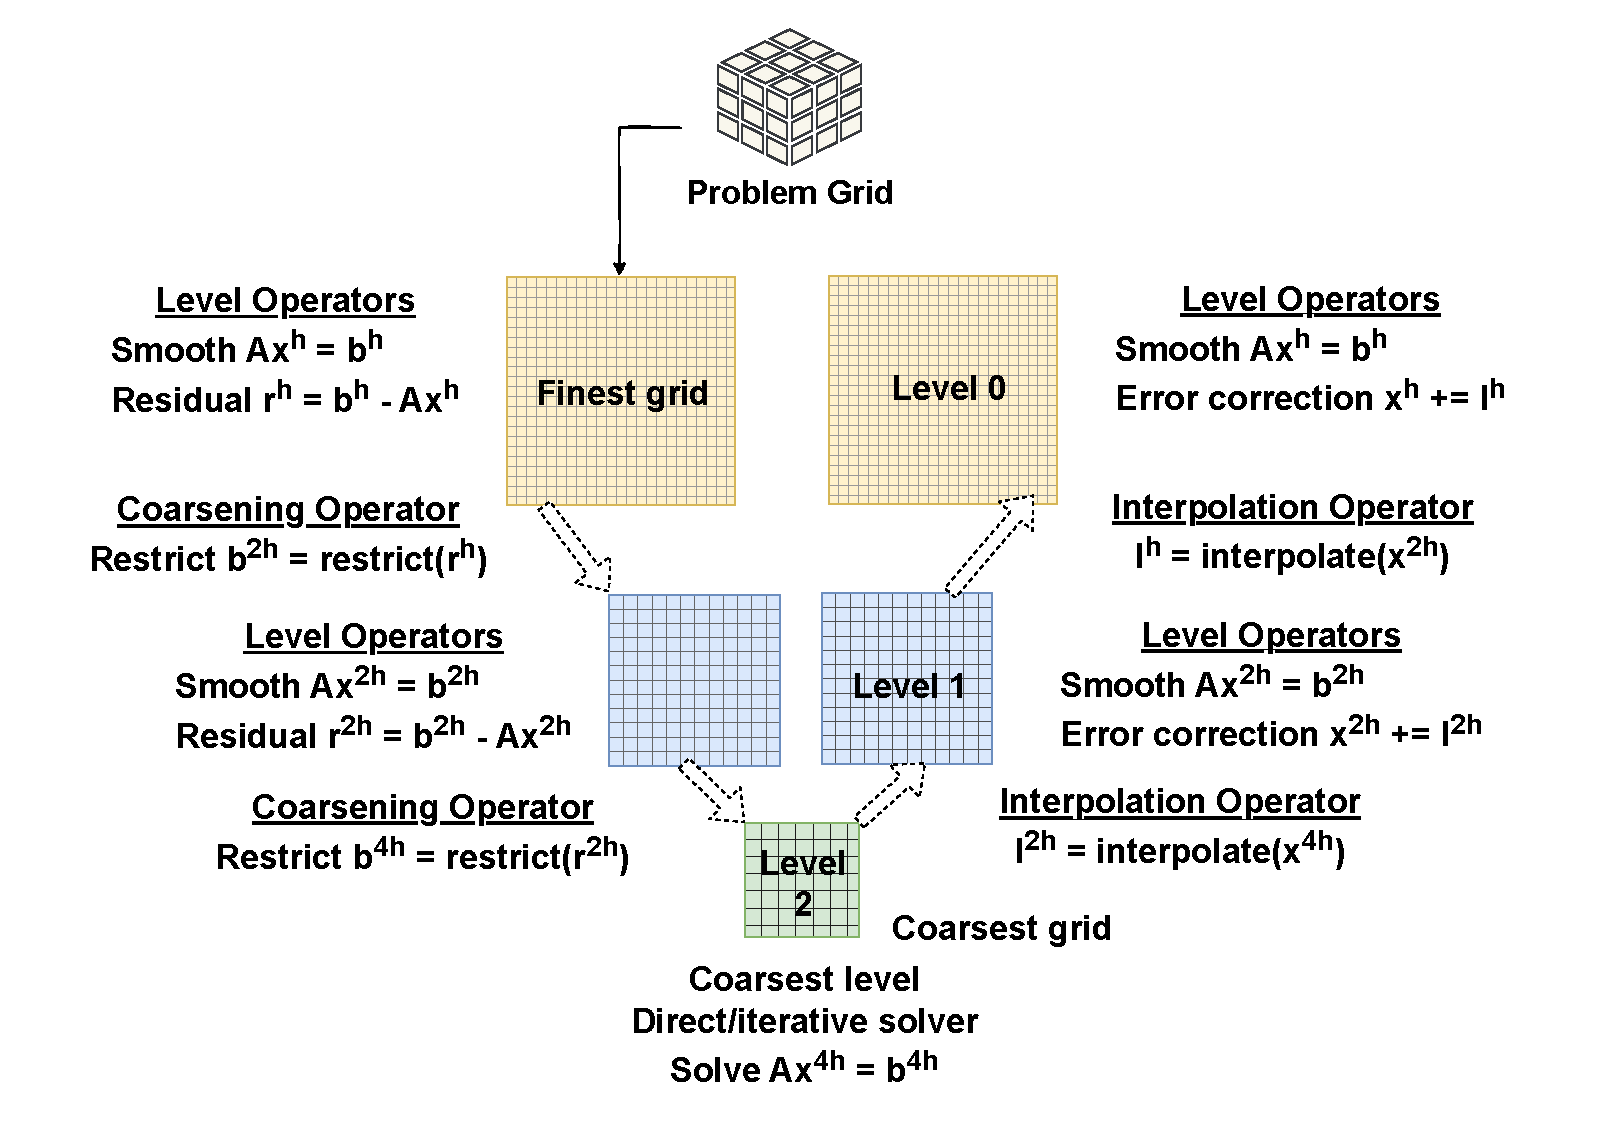
\includegraphics[width=1\linewidth]{fig1_gmg_v_cycle.drawio (5).pdf}
    \caption{Schematic representation of a Geometric Multigrid V-cycle illustrating smooth, restriction, coarse-grid correction, and interpolation operators. Small 3D grid represents the problem domain}
    \label{fig 1:V-cycle in GMG}
\end{figure}

This paper evaluates the implications of mapping GMG to 
the Cerebras Wafer-Scale Engine (WSE), a radically different architectural model~\cite{Cerebras,Lauterbach}. By integrating nearly one million processing elements (PEs) and tens of gigabytes of on-wafer SRAM onto a single wafer-scale chip, the WSE provides single-cycle access to local memory and 21 petabytes-per-second of memory bandwidth, along with 214 petabits-per-second of fabric bandwidth through a 2D mesh interconnect. %This fine-grained distributed-memory architecture eliminates traditional cache hierarchies and drastically reduces memory latency both on PE and across PEs. 
As a result, algorithms that are typically memory-bound on CPUs and GPUs frequently become compute-bound when ported to the WSE.  Prior work has demonstrated this shift for diverse workloads such as stencil computations~\cite{Sai,sai2,Rocki,scalable_25pt_stencil,mathias}, seismic analysis~\cite{Ltaief}, molecular dynamics~\cite{perez_md_sc24,perez-journal}, %Monte Carlo simulations~\cite{Rocki,Ltaief,mathias} 
and Monte Carlo particle transport kernels~\cite{Tramm24,Yoshii26}. % [cite:25-point stencil; others].

%\textbf{Why GMG, Why Stencils, what's the need to choose it?}
%\textcolor{red}{This paragraph also starts out too broad.  Mary edited:}
%Despite these successes in stencils, what remains missing is a demonstration of scientific computing workloads that go a step beyond traditional stencil kernels. 
In this paper, we build on the lessons from successful use of Cerebras for stencil computations to provide a mapping of an algorithm that is
%, while important, are now a well explored class of applications on this dataflow machine, and several efforts have replicated or extended these patterns but yet to address a more realistic, end-to-end use case. From the perspective of the Berkeley “Seven Dwarfs” [citeme] taxonomy, \textit{structured grids} represent a key category of scientific workloads that to our knowledge have not been explored on this hardware, particularly in the context of large-scale PDE solvers. This gap highlights the need to push beyond simple 7-point or 25-point stencils towards workloads that are 
still structured yet significantly more challenging. %Geometric Multigrid (GMG) serves as a manageable proxy application for real-world PDE solvers, %(Adaptive Mesh Refinement(AMR)), 
%while introducing algorithmic complexity that stresses the architecture in %nontrivial 
%several ways. GMG incorporates richer loop structures, multi-level communication, data movement patterns across PEs and in particular different layer mapping strategies, in its smoother, restriction, and interpolation phases. Geometric Multigrid (GMG) exploits the structured hierarchy of the underlying mesh and operates in a matrix-free fashion, relying on stencil computations rather than storing the full sparse matrix, a property that is both memory-efficient(48KB memory) and compute-friendly [cite: PDE \& discretization slides; Sam slides]. 
%\textcolor{red}{The implementation details (like CSL) are too low-level for the intro.  I don't think you should say things like hop-based and window-based either, especially since they are not defined.  This paragraph could summarize the findings, for example: \textit{
As compared to a GPU implementation of GMG, we find that the implementation of GMG must address new challenges on the Cerebras architecture: (1) limitations on problem size that fit on the wafer compared to GPU; (2) relative communication costs growing at deeper levels of the V-Cycle; and, (3) trading off code size and data space in the memory-constrained tile. 
These results suggest several adaptations of the multigrid algorithm to maintain the benefits of low memory latency within the tile and fast nearest neighbor communication.  %such as ??? shallower levels and more like a W-cycle, lower-order of stencil due to less memory, ...???
%In this work, we accelerate the Geometric Multigrid Layers using a distributed-dataflow mapping strategy onto the WSE-3. We have implemented a Geometric Multigrid algorithm using CSL, a low level Zig-based kernel programming language for writing dataflow programs on Cerebras.  Our implementation relies on a hop-based 7-point stencil implementation and a window based reduction pattern. 

This paper makes the following contributions:
\begin{itemize}
\item The first implementation of a multigrid algorithm on Cerebras, to the best of our knowledge.
\item Extensive performance analysis, including \textcolor{red}{Summarize what results are in evaluation.  End with GPU performance comparison.}%strong/weak scaling behavior.\textcolor{blue}{We can't do a strong scaling as we can't fit > 1 Pencil on 1 PE. It's a weak study paper but we should somewhere talk about this limitation. Which might be a good learning to design a new way of mapping or even for hardware vendors to have say something like a shared tile say across a group of 8 PE. Both learning for hardware vendors or programming abstraction designer (in GPUs we say \texttt{\_\_shared\_\_} or \texttt{\_\_reg\_\_} someone can think like this by annotating a tile 'memorytile' or 'onlycompute' tile, todo: Need to place this at proper location}
\item Lessons regarding GMG algorithm configuration suitable for a tiled architecture with limited memory.
%\item A performance comparison
%We compare our results 
%against the baseline HPGMG[citeme], a high performance proxy for multigrids on GPUs along with [oscar work], showing 13$\times$ speedup over a single-node GPU implementation.
\end{itemize}
%Our main contributions are as follows.
%1. 



\section{Background}
This section summarizes the GMG approach and the key aspects of the Cerebras architecture relevant to this study.

\subsection{Geometric Multigrid Methods}

Multigrid methods are iterative solvers which solve sparse linear system of equations by forming a hierarchy of grid levels and iterating across them to %eliminate errors efficiently. 
improve accuracy.  %The key idea is to convert the high-frequency errors from finer grids into low-frequency errors and solve them at the coarsest grid. 
Geometric Multigrid (GMG) specifically uses the geometry of the problem to construct different levels and the grid hierarchy, as illustrated in Figure~\ref{fig 1:V-cycle in GMG}. 
%The finest level contains the largest amount of data and computation, and each successive level typically halves the grid resolution. A GMG cycle begins with an initial approximation on the finest grid and recursively improves it across the hierarchy to generate correct solution.
In the figure, 
%Fig \ref{fig 1:V-cycle in GMG} illustrates 
a three-level V-cycle is used to solve ($Ax = b$), where (A) is the stencil operator, (x) is the solution, (b) is the right-hand side, and superscripts (h), (2h), and (4h) correspond to grid spacings. Each level performs two primary operations: smoothing and residual evaluation. The smoother reduces high-frequency error, commonly with % by approximately solving the equation (\(A^h x^h = b^h\)), commonly used method is 
the weighted Jacobi smoother. %, expressed as \[x_1^h = x + w(b^h - A^hx)\]
%where w is the weighted Jacobi coefficient and \(x_1^h\) explicitly shows the new smoothened value of \(x\). 
The residual operator %computes \[r^h = b^h - A^h x^h\] which 
measures the deviation of the current iterate from the exact solution. The coarsening step restricts the residual to the next level, generating the coarse-grid right-hand side. %\[b_2h  = Restrict(r^h)\]

In finite-volume discretizations, restriction corresponds to averaging the contributions of eight fine-grid cells into one coarse cell, recursively repeated %The algorithm continues this process 
until reaching the coarsest grid, where the system is sufficiently small to be solved with a direct or iterative method such as conjugate gradient, BiCGSTAB or Jacobi. %Common bottom solvers include Conjugate Gradient (CG), Preconditioned CG (PCG), and BiCGSTAB or even a Jacobi smoother. 
After the coarse solution is computed, the V-cycle traverses back up through the hierarchy. Interpolation transfers the coarse-grid correction to the finer grid %using  \[I^2h = Interpolate(x^4h)    >> TODO: Fixme\] Where in interpolate 
such that a single coarse cell is replicated to 8 fine cells, the inverse of restriction. An error-correction step updates the fine-grid solution. % using  \[x^2h = x^2h + I^2h        >>  TODO: Fix me\]
Finally post smoothing reduces any high-frequency errors reintroduced during interpolation. This down-and-up traversal is called a V-cycle, and achieves rapid convergence.
%technique produces rapid convergence, alternative cycles, include W-cycles and F-cycles.
%The most expensive computation in GMG is the sparse matrix–vector (SpMV) multiply that appears in smoothing and residual. In structured-grid problems, this operation is implemented in a matrix-free form using stencil operators one such 3D-7 point Laplacian operator. No explicit matrix is stored, which reduces memory and improves locality. The total time of a multigrid is the number of iterations multiplied by the time for one V-cycle shown in equation (1). 
    The cost of each V-cycle depends on the number of levels, the choice of operators and coarse-grid solver, the number of iterations on the coarse solver, and the performance of the stencil computation. Optimizing GMG therefore requires optimizing each operator %, specifically Stencil operator 
and the interactions between levels.
%\[TimeTotal = iterations * TimePerV-cycle\]
%\textcolor{red}{You need to list all of the operators and their goals}
%\textcolor{red}{The V-cycle should have been at the beginning of this section.  This is late.}
%\textcolor{green}{Todo: Seems like some pieces can be trimmed, dumped as of now}



\begin{figure}[ht]
    \centering
    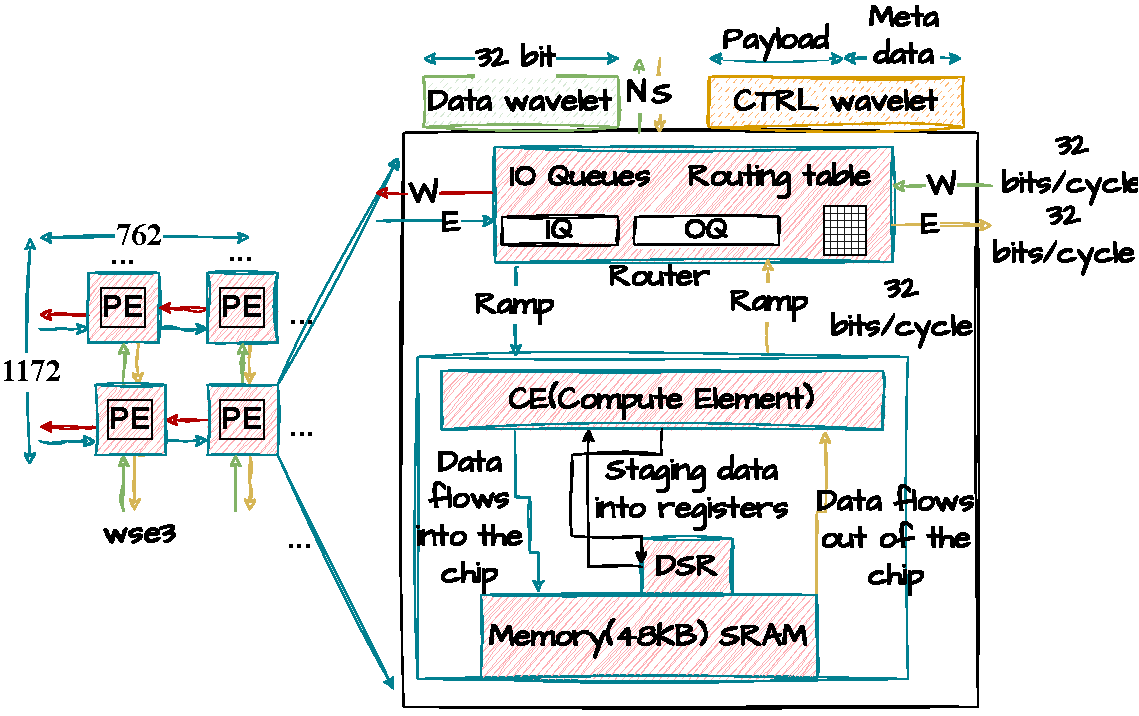
\includegraphics[width=1\linewidth]{adsda.drawio (1).pdf}
    \caption{A schematic representation of WSE-3, %. The WSE is 
    a 2D grid structure where %made up of dies and 
    each die is made of processing elements (figure left). %Figure shows a virtual concept of colors used to design routing paths, 
    Figure right shows the hardware machinery inside a PE: router, memory and  Compute Element(CE). The WSE-3 system is a giant 46,255 mm² chip along with the machinery needed to cool, power and provide I/O.} %\textcolor{blue}{Increased font please check if readable}}
    \label{fig:CS3}
\end{figure}


\subsection{Cerebras WSE-3 and Programming Model}
Figure~\ref{fig:CS3} shows the schematic representation of Cerebras WSE-3 Wafer-Scale Engine. 
The wafer  consists of  893{,}064 identical, simple Processing Elements (PEs) arranged in a homogeneous 11724$\times$762 2-dimensional grid. Each PE is self-contained with its own Memory, Compute Engine(CE) and Router; i.e.,  the WSE is a spatial, distributed-memory, and dataflow-oriented architecture. %PEs don't share data unless communicated explicitly through the fabric. 

\subsubsection{Router}
A 5-port router moves the data across neighboring PEs (East, West, North, South links) and the Compute Element (Ramp link) using 32-bit \textit{wavelets}, the fundamental unit of communication. Routing is defined by 24 static virtual channels, called \textit{colors}.  In Figure~\ref{fig:CS3}, the colors red, blue, green and yellow show the routing of data into and out of the chip from neighboring directions (N,S,E, and W). %along with types of wavelets over a color channel.
A wavelet is assigned to a color, which encodes a routing path across PEs. A router decides, based on the wavelet's color and its configuration, where to send the wavelet.
%of the wavelet and the configuration of router where should the wavelet go next.  
Multicasting replicates the wavelet and send in all directions with zero cost overhead. The router also has some Queues for input output buffering. 
For dynamic or adaptive routing, the system provides \textit{control wavelets}, which include additional metadata that allows routers to update entries in their routing tables and to trigger control tasks. %This enables runtime reconfiguration when static colors are exhausted or algorithmic phases require different communication patterns. The router maintains input and output queues, and supports multicast by replicating wavelets in multiple directions at essentially no additional cost. 
All links operate at 32 bits per cycle.
%\textcolor{red}{I commented out multicast and input/output queues.  We can add back if used later in the paper.}
%\textcolor{blue}{We are using in the optimization, we can add it back now. }

\subsubsection{CE and Memory}
The Compute Element (CE) executes integer and floating-point operations and includes FP16 and FP32 SIMD instructions 
%-like tensor traversal mechanisms[citeme?] 
that enable fast access to local memory. The CE consists of one main thread and up to eight microthreads, each of which may perform computation or handle I/O wavelets; in this way, computation and communication are overlapped.
%which allow computation to overlap with communication allowing each microthread to handle I/O wavelets and thread to perform computation. FP16 and FP32 operations can be issued through wide SIMD execution units, and a
A small set of Data Structure Registers (DSRs) provide lightweight staging of data to/from the local 48KB SRAM, as shown in the figure. %Given no cache hierarchy, performance comes from the data movement of local 48KB SRAM access, and using tensor access patterns to read and write memory efficiently and using SIMD registers shown as Data Structure Registers(DSR) in the figure to stage the data. 
No data cache is needed since memory accesses exhibit %The memory is 
single-cycle latency with 64-bit writes/cycle and 128-bit reads/cycle~\cite{luczynski_reduce}\textcolor{red}{check CS3?}. In total, the wafer has 44 GBytes of on-chip SRAM memory.  %fast SRAM memory on chip.

%\textcolor{red}{This subsection has good content, but should be shorter.  You should focus on things relevant to the paper content.}

\subsubsection{Programming Model}
    %Unlike CPU or GPU programming, which abstract away memory hierarchies or thread scheduling, CSL requires developers to explicitly define both computation and communication. 
    The programming interface, known as the Cerebras Software Language (CSL), exposes both high-level constructs (loops, functions, conditionals) and low-level primitives (Data Structure Descriptors (DSDs), colors for routing, asynchronous tasks, runtime router configuration)~\cite{CSL}. Typically, %like host-accelerator programming models, 
    the host code is written in python where the programmer manages the initial data copy onto the spatial tiles along with allocation of tensors. The kernels written in CSL manage the allocation of data on each PE and the corresponding computations. The layout code written in CSL defines colors, routing across PEs, and lays the kernel code spatially across the million PEs.
    
    A CSL kernel can consists of \textit{functions} and \textit{tasks}; data and control tasks describe dataflow, and execute only after being activated %where tasks are the mechanism to enable dataflow. There are 3 types of tasks: data task, control task and local tasks, these cannot be invoked like function instead can be activated. These Wavelet-triggered tasks(data and control) are activated 
    when a wavelet tagged with a particular virtual channel (color) arrives at the PE’s router, which further can trigger a change in router configurations or perform computations on the data. %, enabling a pure dataflow programming experience. On the other hand l
    (There are also local tasks that must be explicitly activated.) This wavelet-triggered task model offers %high level of 
    asynchronous fine-grained parallelism, but requires the programmer to manage communication and synchronization. %although the programmer has to be careful about managing synchronization across these tasks and not get stuck with deadlocks. To overcome such challenges a task can be blocked or unblocked to explicitly gain control over it's execution. 
    
%\textbf{Motivating para and connect to GMG/MG:}
\subsubsection{Example}
%    Together these features establish an asynchronous fine-grained distributed dataflow model where wavelets serve as messages and colors define communication channels, effectively treating a million distributed PEs as a coherent, programmable network. %\textcolor{green}{By abstracting away the complexity of conventional MPI-style distributed computing}, this paradigm allows developers to program the entire fabric as a single chip while exploiting massive parallelism. However, it demands a careful design and fundamental rethink of data placement, routing and locality; particularly for multilevel algorithms like GMG, where varying computation and communication patterns make spatial layouts and mapping strategies critical to performance.
%Furthermore, collective operations such as row-wise reductions, broadcasts, timers are available as built-in primitives, but developers can also design custom routing patterns in layout files to tailor communication for their specific algorithms. 
%\textcolor{red}{I commented out most of the paragraph that is supposed to connect to GMG, as it does not currently do that.  But I like the suggestion below of a small code example so I left the first sentence.  It could also be deleted.}
\textcolor{green}{TODO: I have idea of a figure with 3 boxes, python, kernel csl, layout csl side by side a small minimal code example?}

\begin{figure*}[t]
\centering
\begin{minipage}[t]{0.49\linewidth}
\centering
        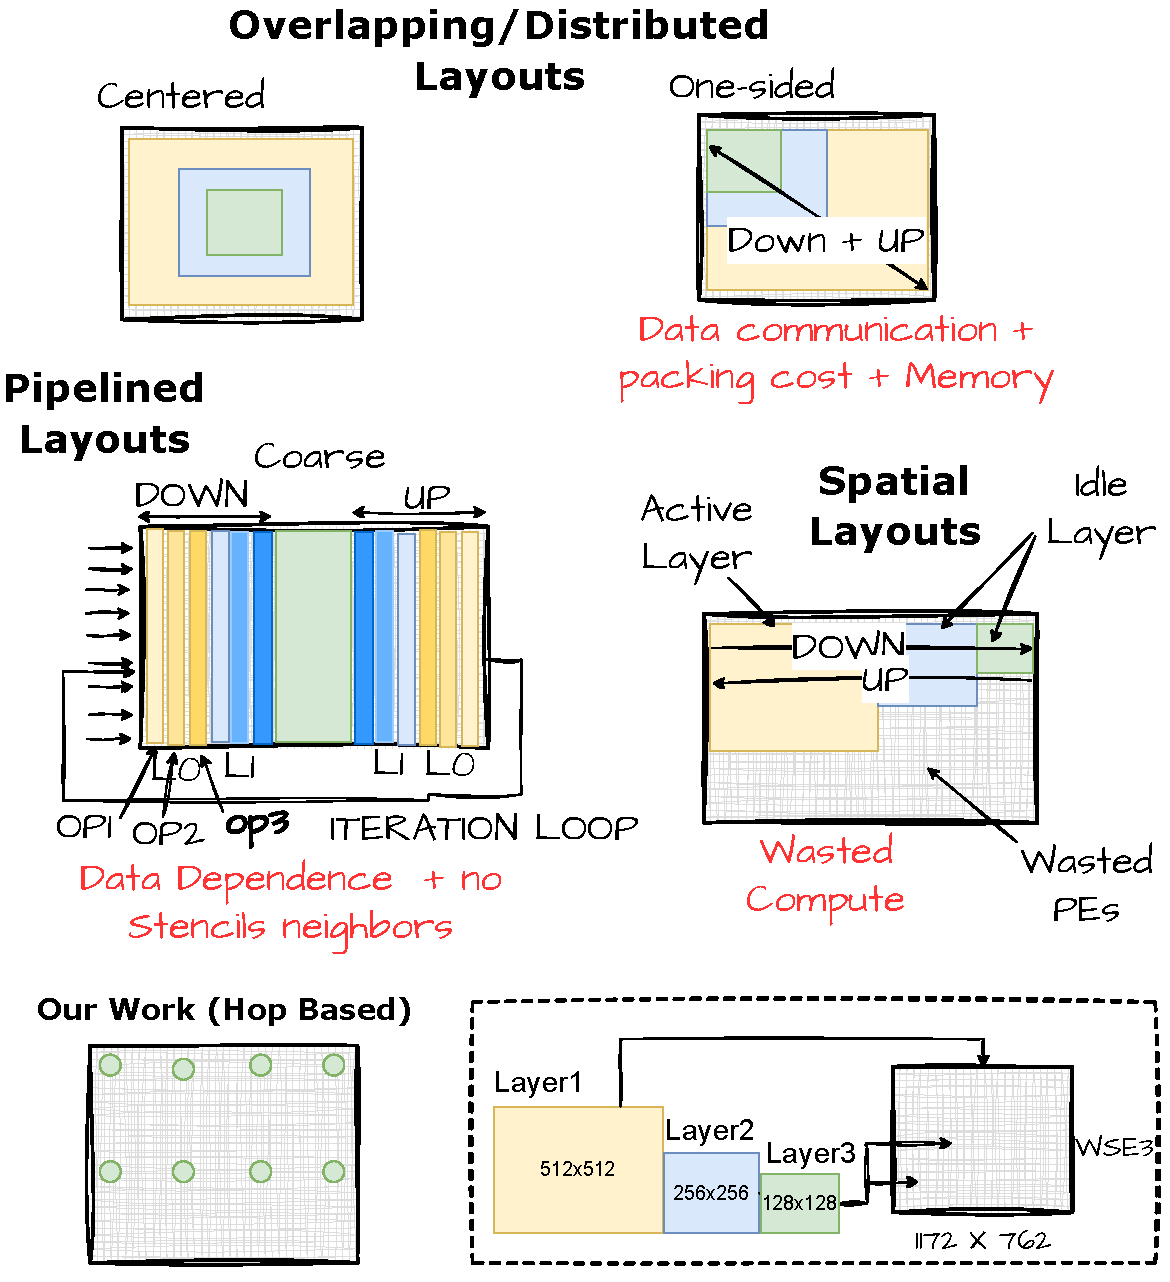
\includegraphics[width=1.0\linewidth]{Copy of layouts.drawio (2) (1).pdf}
        \caption{Different possible layouts for 3 level GMG layers on WSE3 of size 1172x762. Text in red points various challenges of each approach. Our approach falls into the distributed category and we have devised ways to optimize and overcome some of the tradeoffs in our work.  }
        \label{fig:VariousLayouts}
\end{minipage}
\hfill
\begin{minipage}[t]{0.49\linewidth}
    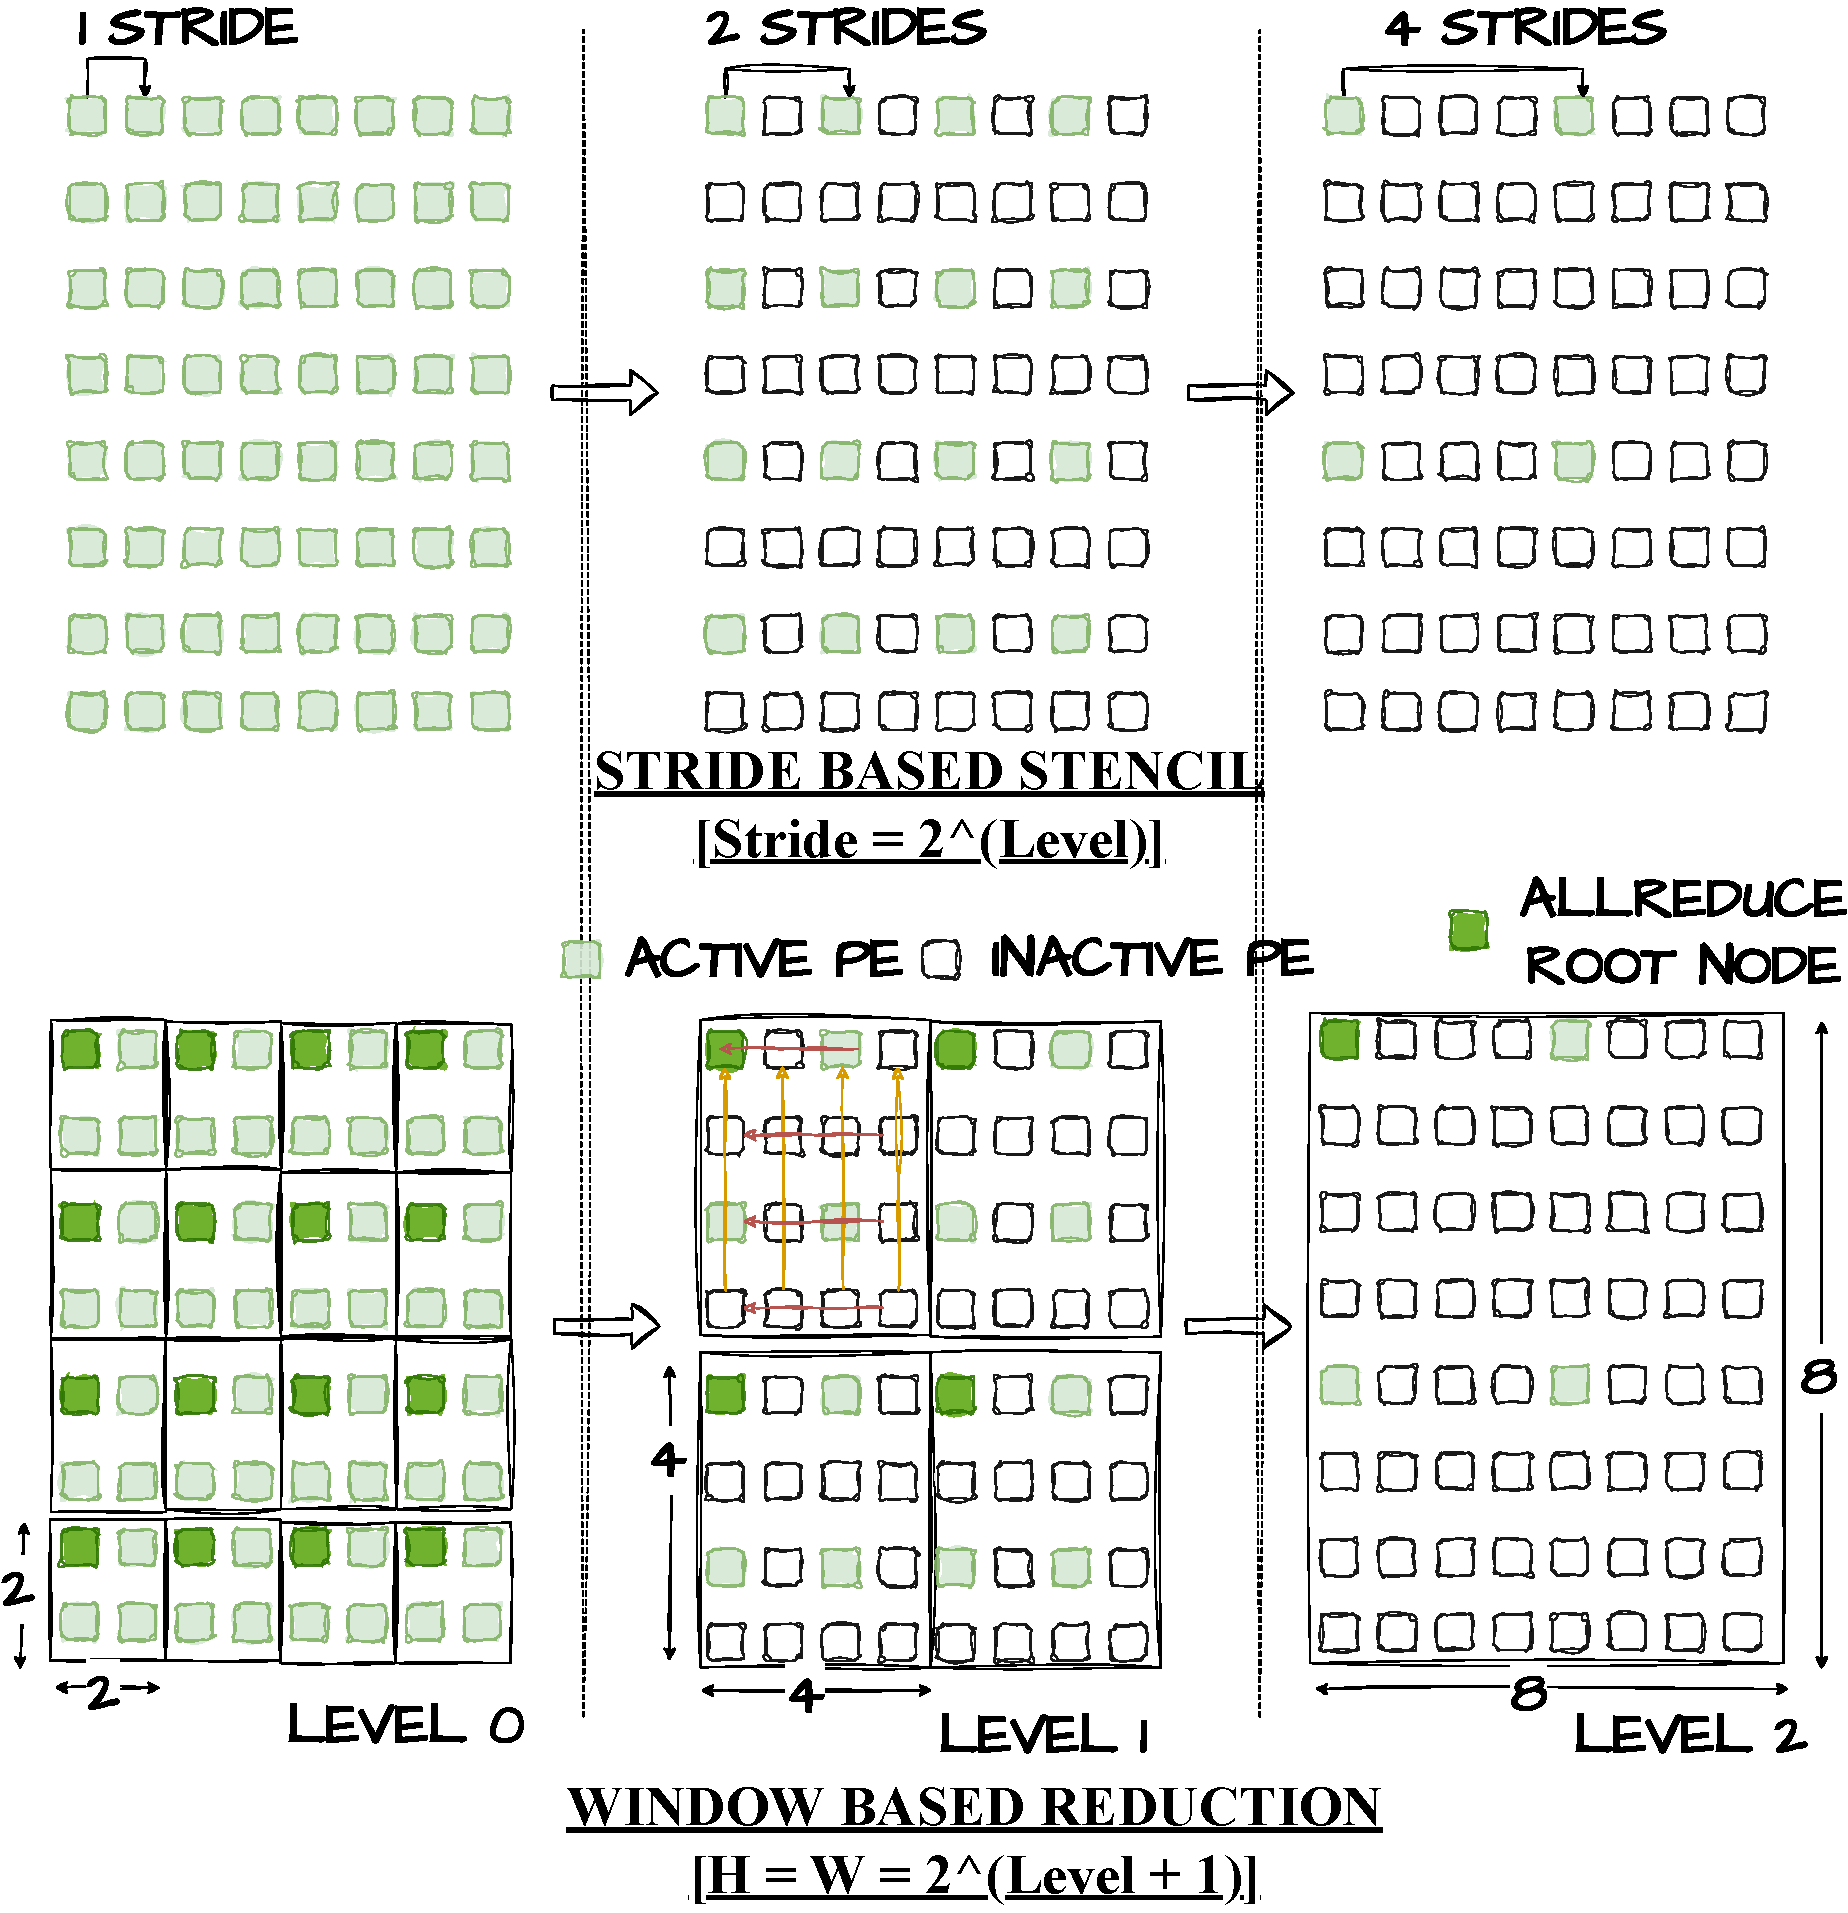
\includegraphics[width=1\linewidth]{stride3.drawio (1).pdf}
    \caption{Top: Stencil Operator performing SpMV on WSE 2D grid for a \(8^3\) problem with 3 levels. The Highlighted nodes are the Active PEs and remaining Inactive PEs. The Hop distance differs as one keeps going down the levels and the SpMV exchanges halo regions H hops apart }
    \label{fig:Spmv_and_restriction}
\end{minipage}
\end{figure*}


\section{Mapping GMG to WSE-3}
    This section describes our mapping of GMG onto the CS-3 wafer.  We consider the pros and cons of alternative approaches of mapping the problem grid and multigrid levels onto the PEs.  We describe the implementations of the operators, and discuss optimization opportunities.
    

    % Compact summary of inter- and intra-level distances for key layout strategies:
    \begin{table}[h]
     \caption{Inter- and intra-level communication distance \textcolor{red}{$D_l$??? -- need to connect to equation 1 terms} for different layout strategies. We assume the intra level distance is the stencil halo exchange neighbor distance and the inter level distance is the maximum distance required between the two levels.}
        \centering
        \renewcommand{\arraystretch}{1}
        \setlength{\tabcolsep}{5pt}
        \begin{tabular}{lcc}
          \toprule
          \textbf{Layout} & \textbf{Inter-level} & \textbf{Intra-level} \\
          \midrule
          Spatial  & $nz_l$ + $nz_l$/2    & 1 \\
          Left-skew-overlapped & $nz_l$  & 1 \\
          Centered-overlapped & $nz_l$/2  & 1 \\
          Strided (this paper) & 2*$2^l$ & $2^l$ \\
          \bottomrule
        \end{tabular}
        \label{tab:layout_comparison_distance}
    \end{table}
    
    \begin{figure}[]
        \centering
        \includegraphics[width=0.7\linewidth]{figures/mapping_max_distance_manhatten.drawio.png}
        \caption{Inter level operator communication distance: The figure shows maximum communication distance a wavelet has to travel between 2 levels across various layouts.This distance is directly proportional to the cost of inter level operators. Note weak scaling can make it possible to reuse the zdim}
        \label{fig:mapping_max_distance_manhatten}
    \end{figure}
    

 \subsection{Alternative approaches for level placement}
    Mapping different multigrid levels onto a spatial accelerator with thousands of independent PEs introduces an interesting design challenge. In addition to domain (i.e., data) partitioning, one has to also perform spatial partitioning and layout of the computation (operators and levels), and routing of data amongst levels. GMG's V-cycle poses unique challenges as the levels have irregular data sizes, and there are data dependences across levels in the iterative algorithm. All of these factors must be considered to arrive at the best mapping strategy. 
    
    In this section, we evaluate different level placement strategies and their tradeoffs: fully distributed, spatial, and pipelined layouts, as shown in Figure~\ref{fig:VariousLayouts}. Each approach has tradeoffs and implications for memory footprint, data communication distance, packing-repacking cost, parallelism, router and coloring code complexities, and amount of chip utilization and power consumption. With the advent of large-scale spatial-dataflow accelerators, one can program the distributed machine as a single device with a single programming model. Therefore it amplifies the importance of placement as routing and communication is directly tied to layout and resulting performance. Therefore, we model the communication cost for different layout strategies and compare them with our proposed strided layout.

    We leverage the performance model %from the near-optimal paper 
    of Luczynski et al.\cite{luczynski_reduce}, which focuses on modeling collective communication operations. We are interested in modeling the inter and intra-level communication costs for each operator, since communication cost is the dominant factor in achieving performance for the various mapping strategies; we omit compute costs as we know they shrink geometrically. 
    
    Per Luczynski et al., Equation~\eqref{eq:comm_model} estimates the number of cycles $T_l$ at level $l$ for a given problem size.   The model has two terms.   In the first term, $C$ is the largest number of wavelets a PE sends or receives, a measure of contention.  $E$ is the total number of hops the network needs to route wavelets; $N$ is the number of links being used (a PE has 5 bidirectional links); and, $L$ is the largest number of hops a wavelet has to travel.  Thus, the first term reflects whether contention or routing the communication pattern is dominant.
    In the second term, $T_R$ is the router-processor latency (multiplied by 2 for sending and receiving data and an additional cycle for storing the received element), and $D$ is the longest pipeline sequence of PEs that perform operations depending on previous calculations.  Combining the two terms provides a model for communication costs %on each other's output.  for.   $P$ is the number of PEs.[TODO:I need to shorten can we reference paper instead?]

    \begin{equation}
        T_l = \max \left( C_l, E_l / N_l + L_l \right) + (2 T_R + 1) D_l
        \label{eq:comm_model}
    \end{equation}

Therefore, for the context of this paper, the data that must be communicated is the pencil resident at each PE for a given level, and the number of hops it must be communicated is a function of the level.  
%we model costs with Equation~\ref{eq:comm_model_2}. \textcolor{red}{What is confusing here is that I think you are trying to apply Equation 1 to your context, and Equation 2 is confusing because it does not directly map.  I think you should omit Equation 2, improve the paragraph describing Equation 1 to be clearer, and use text to describe how Equation 1 applies in this context.  I made an attempt to simplify some of the long names of Equation 2, but I can't figure out how to define all of the terms.  Why introduce $cost_R$ or $PE_l$ rather than use 2$T_R$ and $D_l$?  This model is good, but needs to be cleaner.}
\begin{comment}
    \begin{equation}
        \begin{split}
            T_l &= \max\left( \text{size\_pencil}_l, \frac{\text{size\_pencil}_l \cdot \text{dist}_l}{\text{dirs}_l} + \text{dist}_l \right) \\
            &\quad + \left( \text{cost}_R \cdot \text{PE}_l \right)
        \end{split}
        \label{eq:comm_model_2}
    \end{equation}
    [TODO:] If above eqn is hard to grasp, can remove?
\end{comment}
    Given the structured grids in GMG, we know that the size of a pencil at level $l+1$ is half the pencil size at $l$
    for all types of layouts. \textcolor{red}{We also need to say something about hops.}  %the varying factor is the distance we call it inter and intra level distance, 
    We show in 
    Table~\ref{tab:layout_comparison_distance} and Figure~\ref{fig:mapping_max_distance_manhatten} the inter- and intra-level distance for different layout strategies.  These will be discussed in the context of each potential mapping of the computation below.
   % \textcolor{red}{Explain how this information will be used in the remainder of this section?}
    
\subsubsection{Spatial Mapping}
       Each layer is spatially mapped either next to each other or far apart but connected via data paths. This approach provides a low-per PE memory usage, high locality for stencils as neighbors are 1 hop apart. But it suffers from high repacking and communication costs across layers. The can cause low overall utilization as many PEs remain idle while waiting for neighboring layers to complete. Also the iteration loop becomes an overhead.

\subsubsection{Pipelined Mapping}
        In pipelined layout one can place layers all along the vertical dimension next to each other or even at a finer granularity to pipeline the layers along with their operators shown in Figure~\ref{fig:VariousLayouts}. The wavelets carry intermediate results from one level to the next and keep feeding the pipeline for the next iteration as they exit the other end of the chip. The closest related work we find is in \cite{CereSZ} where they map various compression operators in pipelined fashion. This strategy is useful for data parallel and feedforward kind of workloads. GMG, however, has data dependences from intermediate data which creates a lot of communication overhead on the fabric when transitioning between layers. Some layers/operators can be idle waiting for data from other computationally-expensive layers/operators to finish causing pipeline bubbles and synchronization stalls. Also the PE parallelism is decreased due to dividing layers along the horizontal dimension. The code duplicates and placement and routing implementation might also become complex.

\subsubsection{Distributed Mapping}
        The distributed mapping approach superimposes layers on top of each other, each PE can perform all the operations. The finest level occupies the full region of wafer, while coarser levels are either mapped towards one side or in the center as shown in \ref{fig:VariousLayouts}. The stencils can be highly parallelized given their nearest neighbor interactions for halo exchanges compared to pipelined and spatial approaches. This also avoids the underutilization of the wafer by using the whole wafer. This mapping aligns closely with CS-3's wavelet-triggered dataflow execution model along with static color configurations to overlap communication and computations which can work across layers. One can rely on underlying stencil efforts~\cite{Rocki,mathias}, which are mapped on this device reusing the previous work. However it can likely go out of memory due to superimposing of all data.  This is where GMG’s structured coarsening is advantageous. Because the $z$-dimension shrinks geometrically. However there can be significant data communication costs as the GMG layers get coarser. This mapping could either be skewed to either side or a better approach to minimize distance could be a centered layout.

\subsubsection{Strided Distributed Mapping (this paper)}
        Multigrids typically have more compute and data at the finer grids, so solving them fast is important. Also reducing the inter layer cost is essential. In our strided mapping we keep increasing the distance between layers by powers of 2. Meaning a PE $2^l$ hops apart is the grid point for that level $l$. This reduces the inter layer cost as the distance between layers increases. Instead of moving the complete data we instead making the operators stride aware. 

We summarize our findings in Table~\ref{tab:layout_comparison}. We describe in detail our strided distributed mapping in the next section.
            \textcolor{red}{*With the current spatial systems we can see this trend where we have to decide the right mapping strategy onto the PEs. Unsolved and open problem. Various options autotuning/modelling can be open directions. ?TODO}
    % memory usage/pe, implementation efforts, compatability with stencil library, stencil-locality, inter-level cost, intra-level/repacking cost, idle PEs, coarse-grid sensitivity
    \begin{table*}[t]
        \centering
        \caption{Comparison of layout strategies for mapping GMG to WSE-3.}
        \label{tab:layout_comparison}
        \renewcommand{\arraystretch}{1}
        \setlength{\tabcolsep}{3pt}
 \begin{small}
        \begin{tabular}{@{}lcccccccc@{}}
            \toprule
            \textbf{Strategy} 
            & \begin{tabular}[c]{@{}c@{}}\textbf{Memory-Usage}\\\textbf{/PE}\end{tabular} 
            & \begin{tabular}[c]{@{}c@{}}\textbf{Routing-Color}\\\textbf{Complexity}\end{tabular} 
            & \begin{tabular}[c]{@{}c@{}}\textbf{Stencil}\\\textbf{Library}\\\textbf{Compatible}\end{tabular} 
            & \begin{tabular}[c]{@{}c@{}}\textbf{Halo-Exchange}\\\textbf{Locality}\end{tabular}  
            & \begin{tabular}[c]{@{}c@{}}\textbf{Inter-level/}\\\textbf{Cost}\end{tabular}  
            & \begin{tabular}[c]{@{}c@{}}\textbf{Intra-level/}\\\textbf{Repacking}\\\textbf{Cost}\end{tabular}  
            & \textbf{Utilization} 
            & \begin{tabular}[c]{@{}c@{}}\textbf{Coarse-level}\\\textbf{sensitivity}\end{tabular} \\
            \midrule
            Spatial      & Low & Simple    & Yes  & High  & Low   & High   & Low         & Low      \\
            Pipeline(Recheck this?)     & Low   & Simple    & Yes  & High  & Low   & High   & High         & ?      \\
            Left-skew-overlapped   & High   & High    & Yes    & Good  & Low   & High   & Medium         & Low      \\
            Centered-overlapped & High   & High    & Yes    & Good  & Low   & Medium   & Medium       & Low      \\
            Strided (this paper) & High   & High  & Yes    & Varies  & High   & Varies   & High         & High      \\
            \bottomrule
        \end{tabular}
        \end{small}
        \vspace{1mm}
    
        \textit{Notes:} 
        %``Memory footprint'' considers per-PE storage; ``Routing \& coloring complexity'' reflects implementation effort and configuration overhead; ``Stencil locality'' refers to the spatial proximity of stencil neighbors supporting efficient communication; ``Inter-level'' and ``intra-level'' cost capture data movement between/coarse levels and within a single level, respectively; ``\#Idle PEs'' encodes potential underutilization; ``Coarse-level sensitivity'' relates to mapping efficiency as levels become coarser; ``Repacking cost'' highlights the memory and communication required to move or densify the grid for operator application.
        Note: We are talking about stencils by default in all mapping.  We are also talking about iterations, which adds cost.[TODO:fill]
        \end{table*}

    \subsection{From 3D problem domain to 2D wafer}
    The GMG input domain is a structured 3D \(nx \times ny \times nz\) grid as shown in Figure~\ref{fig 1:V-cycle in GMG}. We map a 3D problem onto a 2D grid by storing the entire z-dimension ($nz$ elements) on each PE for a fixed value of $x$ and $y$; i.e., a \textit{pencil}. Given the 48KB memory on each PE, this decomposition enables us to scale the problem by using more PEs. All data accesses along the $z$ dimension are local and do not require communication. This approach has been studied in previous stencil mappings on WSE~\cite{Rocki,Sai,sai2,mathias} citeme[stencil]. Given the multigrid dimensions halve at each level, we have to maintain in memory multiple \textit{pencils} from different layers as we superimpose layers. The total amount of data that will fit is a function of levels, $L$, and pencil size $nz_l$ for each level $l \in L$. The total allocation $A$ along the z-axis per PE is a finite geometric series with $|L|$ levels and $nz$ the size of the finest-level pencil $l_0$, 
    \[
    \text{Allocation} = nz + nz/2  + nz/4  + nz/8 + ....
    \]
    \[
    \text{Allocation} = nz \left( 2 - \frac{1}{2^{\,l-1}} \right)
    \]
    \textit{Allocation} represents the amount of data that must fit in 48KB memory along with other intermediate vectors and kernel buffers, and the program code for the PE.
    The finest layers in GMG need the highest amount of data and are computationally expensive; therefore, layer $l_0$ requires the most memory.
    \subsection{GMG operators}

    \paragraph{Jacobi and Stencil Operator/SpMV on the Fabric}
    On GPUs, SpMV struggles with irregular memory access. On the WSE, values are fetched from deterministic SRAM addresses. Communication of off-diagonal contributions is expressed as neighbor packet sends. This makes SpMV effectively a streaming stencil operation, aligning well with wafer-scale execution.
    Figure 4: SpMV as streaming stencil on WSE.
    (Placeholder for diagram: each PE loads local vector, exchanges halos with four neighbors, computes local output.)

\subsubsection{Restriction and interpolation on the Fabric}

    \textbf{c ) Residual/}
    d) Extra: Rho check and setup

    OTHER IMPORTANT POINTS:
    1. How is data dependencies problem solved: 
        We save data during down cycle and recover it during up cycle. Here we can talk about DSDs, SIMD and why we need to save data and when to recover. 
        
        % \begin{figure}
        %     \centering
        %     \includegraphics[width=0.60\linewidth]{DSD_save.drawio.png}
        %     \caption{Layout of data from all layers in memory of a single PE. The total size is Geometric Series of ZDim and Levels(L)}
        %     \label{fig:Flatmemory_layout}
        % \end{figure}
        
        

        var save\_u\_smooth = @zeros([TOTAL\_GMG\_SIZE]f32);
        var save\_f\_down = @zeros([TOTAL\_GMG\_SIZE]f32);
        Pros: Memory is consumed a lot!
        Cons: We can track the data back when going up the V cycle and make algorithm work. 
        

    2. V cycle execution:
        Talk a little about the state machine implementation and why we need it, show various states if needed, talk about synchronization and how we ensure it using the state machine and callback mechanism.
        
    3. How memory problem is solved? Not solved, we have this issue, although we try to then optimize how we can fit 512. 
            * inlining
            * Code size experiments
            * data size, Stencil halos halved for largest problem sizes.
            * Remove unnecessary code from libraries and our code base. 
            * Teardown phase taking so much uncontrollable code. 

    4. How stencil problem is solved? 
        * We use localized stencils we have ability to talk to neighbors.
    5. Wasted compute: Yes we do as well waste a lot of compute but we can scale across wafer and can do so called Wafer scale computing. 
    6. How we solve data communication problem/packing - We avoid those problems as we don't move data instead we adapt algorithm. 
    7. Optimization: 
        SpMV : Skip inactive nodes, coloring changes, control wavelet and change in coloring layout pattern.
        Memory , inlining, code size and data size
    8. 

    \subsection{V-Cycle Execution}

    The V-cycle requires coordination across levels: Fine-level smoothing is aynchronous and parallelized across all PEs. We sync all PEs before to make sure timers are synchronized. The implementation is a state machine with various states as a way to synchronize between the operations.
    SMOOTHING:
    1. STATE_DOWN_INIT          <--- Setup the window based and stride based parameters
    2. STATE_DOWN_SMOOTH_APPLY  <--- Ax_1 = 7_pt_stencil(A, x)
    3. STATE_DOWN_SMOOTH_UPDATE <--- x_smooth = x + Ax_1
    RESIDUAL:
    1. STATE_DOWN_RESIDUAL_APPLY    <--- Ax2 = 7_pt_stencil(A, x_smooth)
    2. STATE_DOWN_RESIDUAL_COMPUTE  <---   r = b - Ax_2
    RESTRICTION:
    1. STATE_DOWN_RESTRICT_ALLREDUCE <--- b = window_based_reduce_into_top_left_PE(r)
    2. STATE_DOWN_RESTRICT_DIV       <--- b_next = b/8
    INTERPOLATION:
    1. STATE_UP_INIT                <--- Setup the level and restore the dependent data from down cycle
    2. STATE_UP_EXPAND_Z            <--- x_coarse = expand_dimensions_local(x_fine)
    3. STATE_UP_BCAST               <--- I = broadcast_from_top_left_PE(x)
    ERROR-CORRECTION:
    1. STATE_INTERP_ADD             <--- x = x_smooth + I

\section{Evaluation}

\begin{comment}
{\color{blue}
\textbf{Outline:}
\begin{enumerate}
    \item[1.] Missing experiments: Roofline and power draw numbers.
    \item[2.] Description of figures and tables and cross references<missing>
\end{enumerate}
}
\end{comment}

%Cleaned up to use acronyms already defined.  
In this section, we evaluate the performance of %Geometric Multigrid (GMG) 
GMG implemented on the Cerebras WSE-3 %Wafer-Scale Engine 3 (WSE-3) 
and compare it against the state-of-the-art %GPU implementation using the 
HPGMG (High Performance Geometric Multigrid) GPU benchmark. %, %[citeme]  an open-source benchmark used for standard ranking and benchmarking of supercomputers on NVIDIA GH200. 
%All results focus on weak-scaling behavior, which is dictated by per-PE memory constraints and the chosen mapping strategy.

% I don't understand why you are using \subsection*???  This will be problematic for final manuscript and does not look different.
%\subsection*{A. Experimental Configuration}

\subsection{Experimental Configuration}
%In these experiments, w
We used the CS-3 cluster in the Argonne National Laboratory Compute Facility (ALCF), which
%the machines at Argonne National Labs[HIDE?]. The CS-3 cluster at ANL[HIDE?] 
consists of 4 WSE-3 machines along with proprietary memory nodes called MemoryX. %as a part of cluster[cite alcf machines]. 
One WSE-3 wafer integrates 893,064 processing elements (PEs) arranged in an 1172 $\times$ 762 2D mesh operating at 875 MHz along with 44 GBs of total on-chip SRAM memory. We used Cerebras SDK version 1.4.0 [https://sdk.cerebras.net/installation-guide]. The experiments were conducted on a single WSE-3 %as accelerator 
attached to a host with Linux kernel 4.18.0 running on an AMD EPYC 9354P 32-Core Processor with 188 GBs of main memory. For the GPU baseline comparison, we used an NVIDIA Grace Hopper GH200 with 120GB of RAM running CUDA 12.8. \textcolor{red}{To be consistent, you may want to say where the H200 node is housed.} We modified the baseline HPGMG code \textcolor{red}{[citeme baseline code github]} 
to use single precision data as WSE-3 does not support double precision.
The backend CSL compiler has the following options: \texttt{--llvm-option=--inline-threshold=256 --llvm-option=--unroll-threshold=256}. \textcolor{red}{What compiler/flags did you use for GH200?} To ensure a fair comparison, we run the GH200 GPU and WSE-3 using identical configuration parameters.

%\subsection*{B. Problem Description}
\subsection{Problem Description} 
We evaluate the performance of GMG %a geometric multigrid (GMG) algorithm along with convergence checks 
implemented entirely on the device. All experiments solve a 3D finite-volume problem \textcolor{red}{[OSCAR? correct?]} on a structured grid using a standard 7-point stencil. The domain is discretized uniformly in all three dimensions, and homogeneous Dirichlet boundary conditions are imposed on domain boundaries with stencil operations applied only on interior cells. The grid spacing of $h^2$ is uniform in all three dimensions. 

%\textcolor{red}{The following paragraph is hard to read -- a lot of detail and formulas inlined into the text.  Perhaps you could put the configuration information into a table?}
The right hand of Ax=b is initialized to: 
\begin{center}
$f(x,y,z)=\sin(\pi x)\sin(\pi y)\sin(\pi z)$\\ 
\end{center}
The initial solution $x$ initialized to 10.0, and the stencil coefficients are: $\alpha = -6.0$, $\beta = 1.0$. Jacobi relaxation with $\omega=2/3$ is used as the smoother. The coarsest level goes to a domain size of 2x2, except for shallow V-cycle experiments. Convergence is determined based on the maximum norm of the residual at the finest level, and solver iterations terminate once a prescribed tolerance($\epsilon = 10^{-5}$) is reached or a maximum number of V-cycles is reached. 

All timing measurements are collected on-device using hardware counters and excludes host-to-device and device-to-host transfers. We report total time per V-cycle as well as a breakdown of time spent in various operators. All experiments are performed in single precision (FP32) arithmetic. We show various experiments that change the number of pre-smoothing and post-smoothing and coarse-smoothing iterations at the coarsest level. Unless otherwise stated we show the experiments with 6/6/6(pre/post/coarse) as the default configuration as that turns out to be the best-performing configuration for GLOW. The hardware uses 16 channels, and 256 block size, as explained in 
%(See Section 
Section~\ref{sec:impact-of-optimizations-and-memory-constraints}. \textcolor{red}{Where is this explained?  Why 256 and not 512?} %as to why we choose the size). 
%This is being moved to the configuration paragraph.  It is out of place here.
%The backend CSL compiler has the following options:"--llvm-option=--inline-threshold=256 --llvm-option=--unroll-threshold=256".To ensure a fair comparison, we run the GH200 GPU and WSE-3 using identical configuration parameters.

The maximum problem size (using powers of 2) that fits on the WSE-3 is $512\times512$ because of the small
%under our current mapping and the 
48\,KB per-PE memory limit, which must store code as well as data.  %we cannot scale beyond a $512\times512$ PE grid. Limiting our experiments for larger problems.

%\subsection*{C. V-Cycle Performance and Operator Breakdown}
\subsection{V-Cycle Variation Performance Comparison}
    Figure~\ref{fig:hpgmg-speedup} reports the performance of GLOW on WSE-3 compared against HPGMG on NVIDIA GH200 bars above the speedup of 1 baseline bar mean WSE-3 is faster. %showing relative speedup where values above one indicate that WSE-3 is faster. 
    The $x$-axis denotes the 2D PE grid size under weak scaling; the $z$-dimension of the problem maps one-to-one onto the grid, so larger grids correspond to larger 3D problems. Each bar in a group corresponds to a distinct multigrid configuration experiment, parameterized by the number of pre, post, and coarse-level smoothing iterations. GLOW consistently outperforms HPGMG on the GH200, with speedups increasing as problem size scales. The best speedup, approximately $25\times$, is observed at the $512\times512$ grid for the $6/6/6(shallow)$ configuration. In contrast, configurations with aggressive coarse-level smoothing, such as $4/4/100$, show the lowest speedups, particularly at larger grid sizes of $256x256$.

% Move this figure here to ensure it appears immediately before the following paragraph,
% not at the top of the page.
\begin{figure}[h!]
    \centering
    
\includegraphics[width=0.95\linewidth]{figures/hpgmg_speedup_barplot.pdf}
    \caption{Speedup comparison between Cerebras CS-3 and Nvidia GH200 using HPGMG/Glow across various problem sizes. The bar plot shows relative performance (higher is better).}
    \label{fig:hpgmg-speedup}
\end{figure}

    %Several trends explain these results. 
    These performance trends highlight the sensitivity of %multigrid 
    GMG performance on WSE-3 to V-cycle structure. Increasing the number of coarse-level iterations (*/*/6 vs. */*/100) along with depth of the V-cycle %deepens the V-cycle and 
    expands communication distances for both inter-level transfers and intra-level stencil operations. %eventually slowing the solver(We analyze the performance in section \ref{sec:operator-breakdown} in detail). 
    In contrast, our implementation handles finer grids well by scaling the problem over the wafer and exploiting parallelism and stencil locality, with shorter communication distances for halo exchanges and fewer hops to travel for inter-layer communication. A $6/6/6(Shallow)$ V-cycle with 7 levels outperforms a $6/6/6(Deep)$ V-cycle with 9 levels by almost 45\% on the largest problem size, with the cost of increased iterations to reach convergence. 
    
    As a second observation, speedups grow as problem size scales. GLOW is well suited to finer levels and larger grids, while single-node GPU performance %tend to struggle on 
    worsens on larger problems due to increased data movement through the memory system. %. as the amount of computation on finer grids grows, factors such as data movement costs and memory bandwidth pressure can also become a bottleneck on GPUs at larger grid sizes. 
    %This sentence belongs in the configuration discussion
    %Third, under our current mapping and the 48\,KB per-PE memory limit, we cannot scale beyond a $512\times512$ PE grid. Limiting our experiments for larger problems.

The configurations with a heavy number of coarse solver iterations (i.e., the blue and orange bars) exhibit a U-shaped trend \textcolor{red}{in Figure~\ref{fig:hpgmg-speedup}???}, as the cost of the coarse solver dominates for larger problems, pushing the performance to lower levels. Configurations with lighter coarse solver iterations (green and red bars) show a linear increase in performance as the problem scales since very less time is spent on the coarse level. A higher bump on the 512 problem size could also point to how baseline\/GPUs start struggling with larger grids and not GLOW performing better by 2$\times$ over previous level.
\textcolor{red}{I'm having trouble understanding this.  The U shape for blue and orange shows improvement on both end points although speedup is low.  Maybe be more precise than saying "U-shaped"?}
    
%\subsection*{D. Operator Breakdown}
\subsection{Per-Operator Performance Breakdown}
We attribute the time spent to 
    %We analyze the performance of 
individual operators in Figure~\ref{fig:per-operation-timing}. %to further explain these results. 
The plot shows time per operator for one V-cycle on a $512^3$ problem, summed over each horizontal level (both down and up phases combined). The $x$-axis is the multigrid level from 0 (finest) to 8 (coarsest); the $y$-axis is execution time in a log scale (higher is slower). %We explain each line in turn.


\textbf{Smooth with 7-point (strided) stencil.}
%\paragraph{Smooth with 7-point (strided) stencil}
%\textbf{Smoothing (7-point hollow stencil).} 
%\textcolor{red}{Using "hollow" everywhere is confusing.  It doesn't start out "hollow" -- I prefer the word "strided".  The stride gets larger as the levels increase. I'm commenting out your text, and trying with my own to make this clearer.  Also, it is premature to compare performance to the residual operator that has not been presented.}
%The smoothing operator, internally implemented using a 7-point hollow-stencil, exhibits behavior similar to that of the residual operator, but with consistently higher cost due to multiple pre and post-smoothing iterations and fixed overheads. As expected, smoothing time initially decreases toward coarser levels because both the number of active PEs and the local data volume are halved at each level. However, unlike conventional weak-scaling behavior reported on CPUs and GPUs[oscar work cite, some GMG CPU/GPU papers] where performance often plateaus/saturates or improves monotonically toward coarser grids, in GLOW we observe a gradual increase in cost beyond a certain level. 
The smooth operator is a 7-point stencil.  At levels above Level 1, strided refers to skipping PEs in the calculation as a result of the grid coarsening.  
As is typical in GMG, smooth time initially decreases toward coarser levels because both the number of active PEs and the local data volume are halved at each level. However, unlike conventional weak-scaling behavior, %reported on CPUs and GPUs[oscar work cite, some GMG CPU/GPU papers] 
where performance often plateaus/saturates or improves monotonically toward coarser grids, in GLOW we observe a gradual increase in cost beyond a certain level. 
        
To better understand this behavior, we microbenchmarked the strided stencil kernel used 
at the heart of the smooth and residual operators, as 
shown in Figure~\ref{fig:spmv-internal}. We measured compute time to calculate the laplacian across the x-y plane and z-axis. %Whereas 
Communication time is the time taken to send and receive halo regions to and from neighbors from all 4 directions. Compute time decreases nearly by a factor of two per level before flattening, due to fixed overheads. Communication cost starts lower than compute on finer grids as the stencil halo neighbors are exchanged directly between neighbors as the machine was designed, while the data size is largest and has maximal computation.
%in the best possible locality and both asynchronous, although the data size is larger leading to higher compute costs. 
The intersection point of these curves reflects the tradeoff between shrinking data volume and increasing communication distance: although each PE processes less data, messages must traverse longer paths as the active region contracts.

{\textcolor{red}{FIX, CLARIFY:
One possible factor is the growing number of inactive PEs towards coarser levels in our mapping. Our implementation uses one input and output microthread for asynchronous fabric communication, along with a main thread responsible for moving data between input and output queues at the router level. 
For inactive PEs, we short-circuit these queues to avoid unnecessary memory accesses. While this optimization eliminates ramp traffic and memory access costs, it can introduce read-after-write (RAW) hazards on the main thread, stalling the main thread, and leading to pipeline bubbles and increased latency.
       }} 

\textcolor{red}{MARY COMMENT: I find this too speculative, and it seems like it is in the wrong place.  Shouldn't you describe this short-circuiting in the "Mapping" section?  And then the rest of this would be there as an alternative.  But if the "color teardown" is not published work by others, don't mention it.  That's why I commented it out.}
One could use control wavelets and runtime coloring reconfiguration as done by Mathias et al.~\cite{mathias} to perform this optimization. %at the color config and routes level. 
%I don't know what this means, and I don't think it contributes
%Another possibility is to teardown the colors before setting each level leading to higher usage of colors which is a limited resource. 
%We took a simpler approach to short-circuit the queues instead as the cost of resetting the colors and reconfiguring the routes might have been higher summed up over V cycles and iterations.
    %We ran the upstream SDK 7-point stencil (hop-based) and saw similar trends with the turning point shifted toward finer levels.
    
    \begin{figure}[h!]
        \centering
        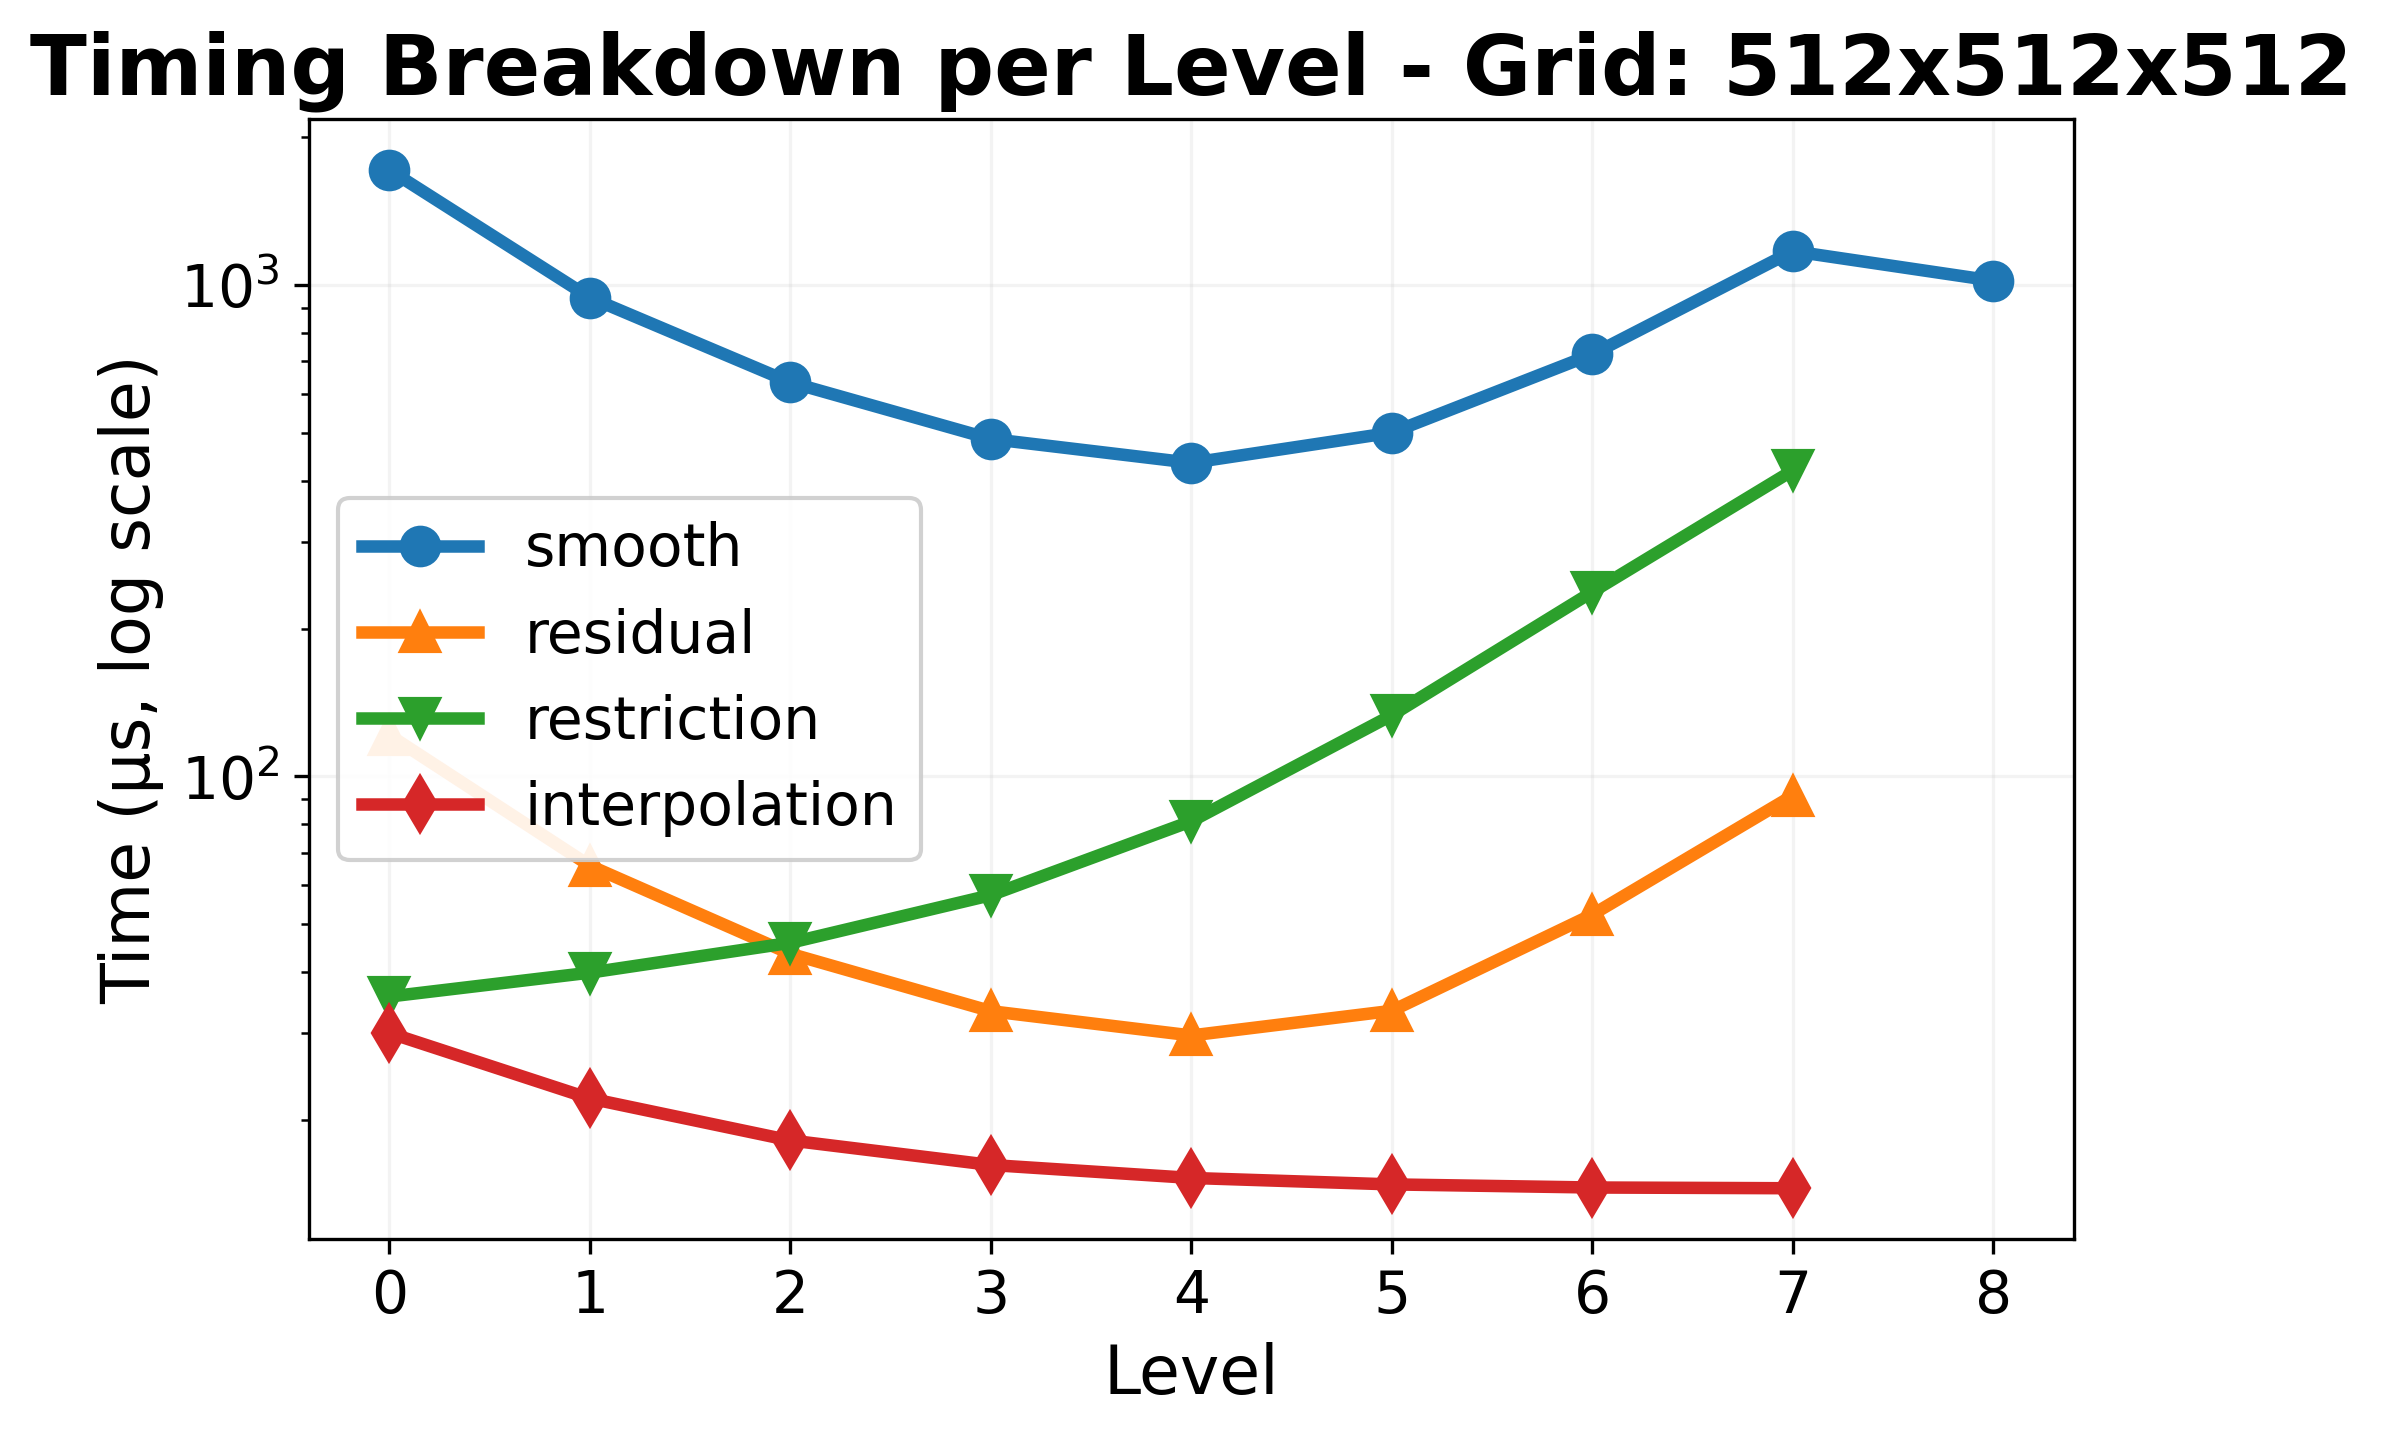
\includegraphics[width=\linewidth]{figures/per_operation_timing_512x512x512.png}
        \caption{Per-operator time per level for one V-cycle on a $512^3$ problem (GLOW on CS-3). Down and up phases are summed at each level. $x$-axis: level 0 (finest) to 8 (coarsest). $y$-axis: time (log scale; higher is slower). Config: $4/4/6$ pre/post/coarse, 9 levels, FP32, 7-point stencil.}
        \label{fig:per-operation-timing}
    \end{figure}

    \textbf{Residual.} The residual operator uses the same 7-point stencil as smoothing and follows a similar performance trend. Differences in absolute time come from the absence of multiple smoothing iterations.

    \textbf{Restriction.} Restriction exhibits increasing cost toward coarser levels. The window-based reduction (Figure~\ref{fig:Spmv_and_restriction}) technique used in our distributed mapping requires contributions from $N-1$ other PEs within a window, introducing dependence and repeated accesses to local memory via the ramp. As the window size grows relative to the number of active PEs, these dependences dominate execution time. Skipping inactive or out-of-domain PEs during the reduction could potentially reduce this overhead and can be a promising direction for future optimization.

    \textbf{Interpolation:} Interpolation shows the opposite behavior compared to restriction; it is more expensive on finer grids and becomes progressively cheaper toward coarser levels. As microbenchmarked in Figure~\ref{fig:interpolation-internal}, interpolation cost is dominated by sending data compared to computing locally. Although one might expect the cost to increase with distance, instead interpolation benefits from the hardware’s zero-cost multicast capability. Data is broadcast in all four directions simultaneously, allowing row-wise and column-wise transfers to occur in parallel. Unlike restriction, interpolation lacks producer-consumer dependences between PEs, enabling immediate forwarding without intermediate memory accesses, meaning each PE can multicast and advance, thus avoiding the high cost of going down the ramp to memory. As the data volume shrinks at coarser levels, smaller packets are sent over longer distances, but the use of multicast and the avoidance of ramp traffic result in lower overall cost. In Figure~\ref{fig:interpolation-internal}, we see that at each level the window-leader PE (top-left, as shown in Figure~\ref{fig:Spmv_and_restriction}) expands the z dimension, resets the routes, broadcasts data, and eventually when data reaches the destination, calculates the error correction locally using tightly coupled DSD operations. Notice the cost to reset routes is constant mostly.

    % SPMV internal:
    \begin{figure}[h!]
        \centering
        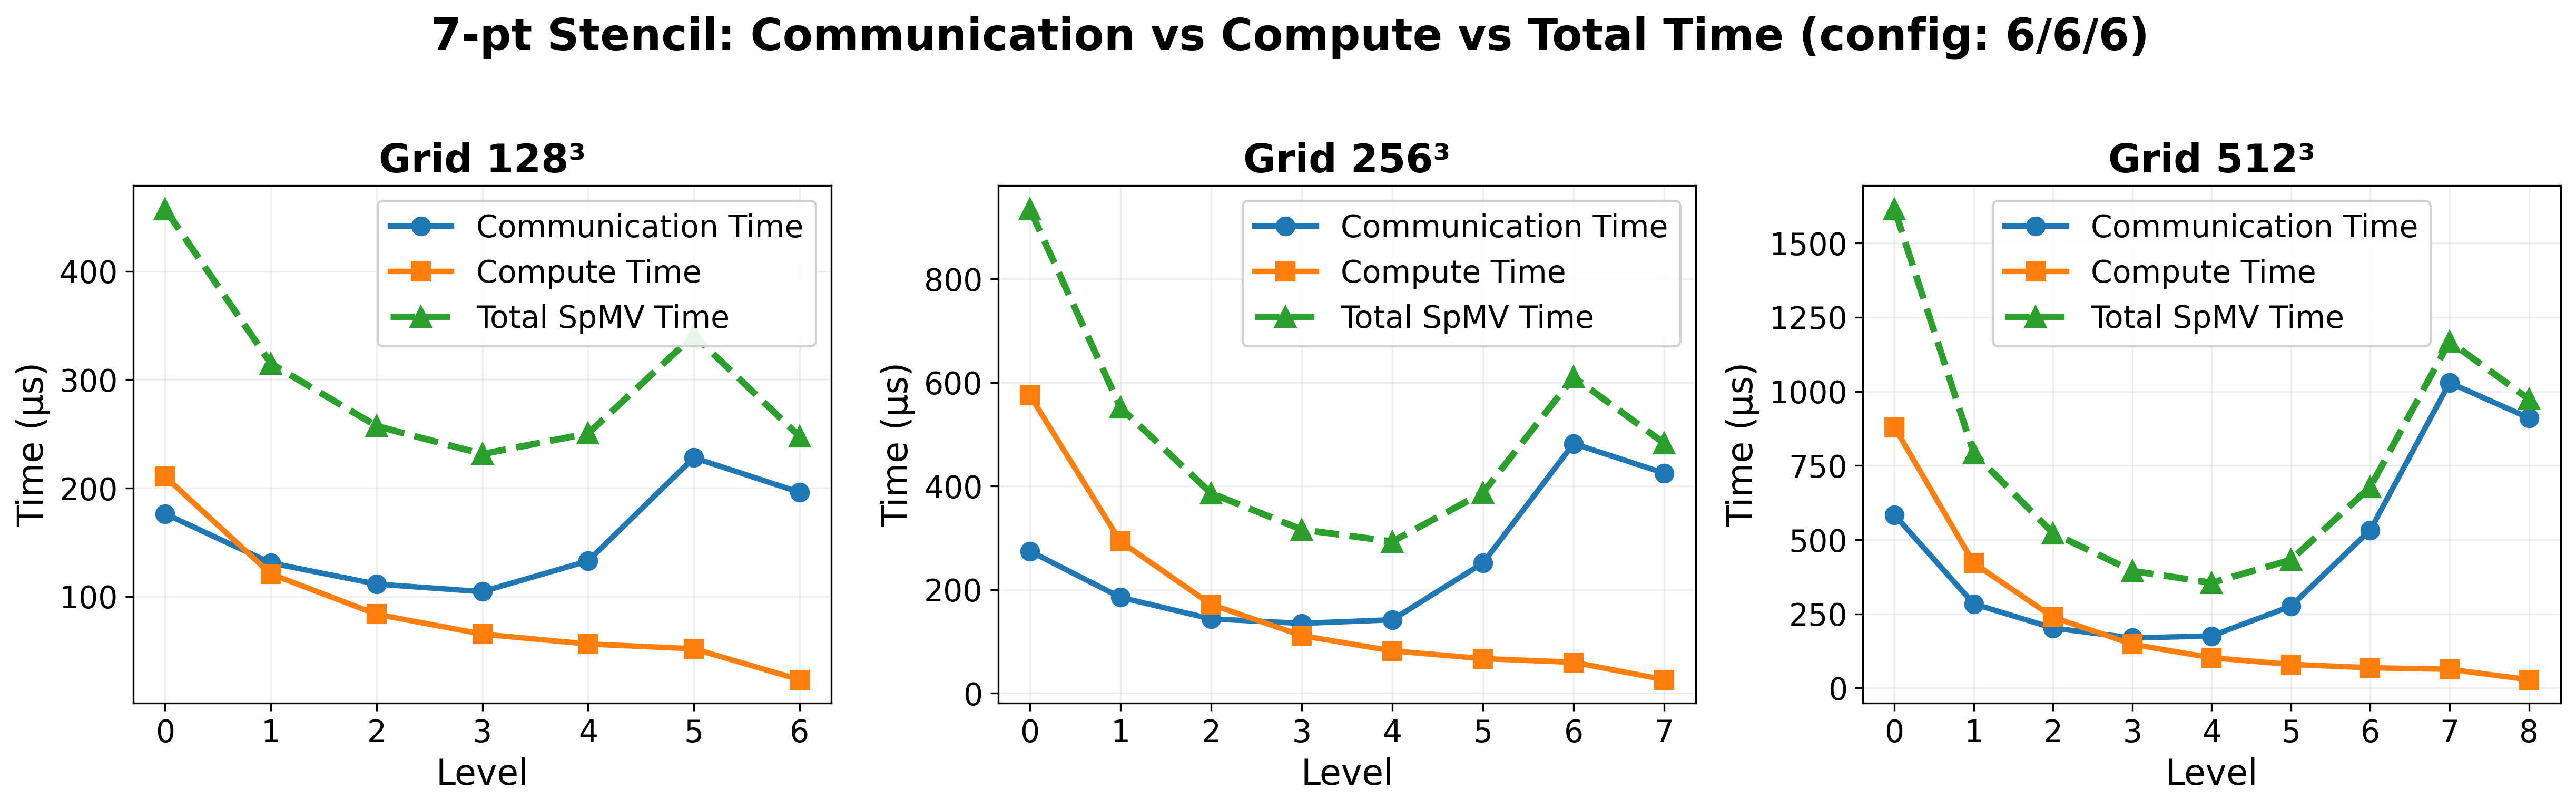
\includegraphics[width=\linewidth]{figures/spmv_internal.png}
        \caption{Internal speedup of smooth on Cerebras CS-3 and Nvidia GH200 using HPGMG and GLOW across various problem sizes. The bar plot shows relative performance (higher is better).}
        \label{fig:spmv-internal}
    \end{figure}

    % interpolation internal:
    \begin{figure}[h!]
        \centering
        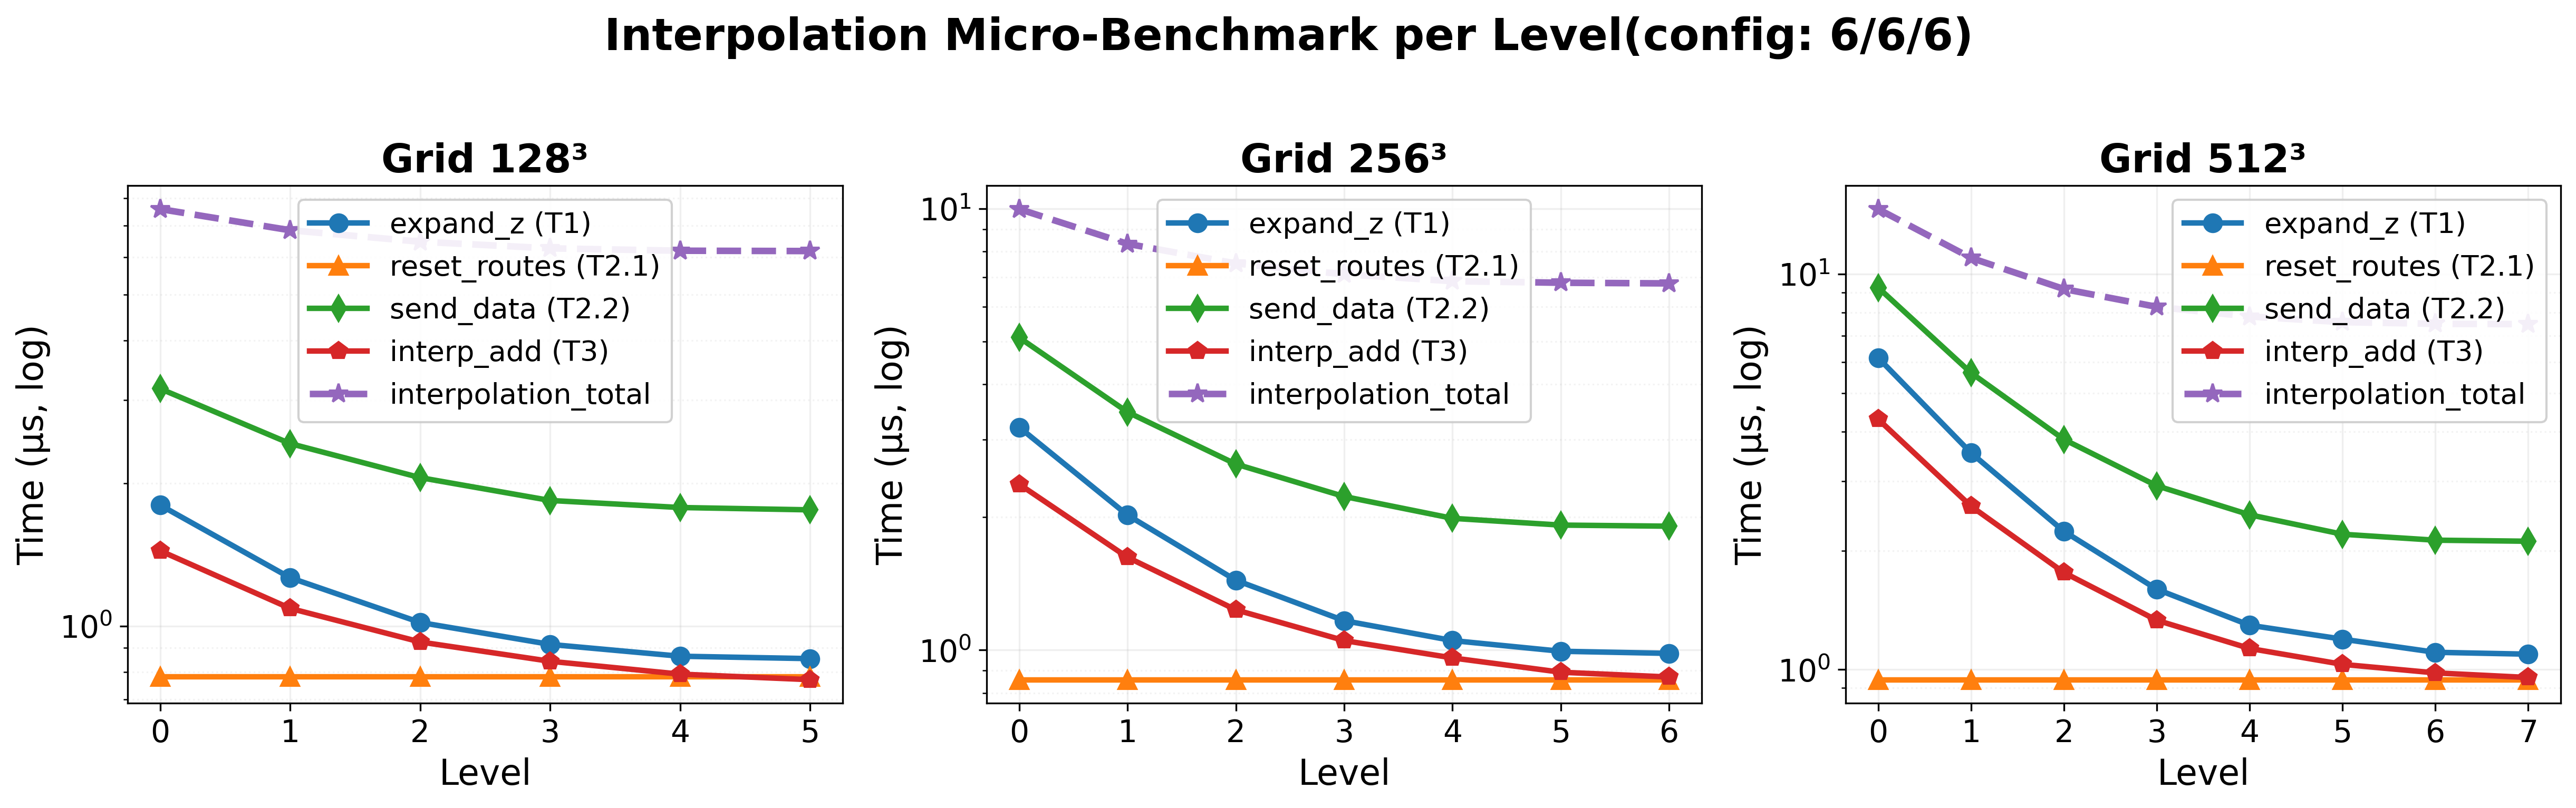
\includegraphics[width=\linewidth]{figures/interpolation_internal.png}
        \caption{Internal speedup of interpolation on Cerebras CS-3 and Nvidia GH200 using HPGMG/Glow across various problem sizes. The bar plot shows relative performance (higher is better).}
        \label{fig:interpolation-internal}
    \end{figure}

    \textbf{Coarse solver.} The coarse solver applies weighted Jacobi relaxation on the coarsest grid. Its cost is very high compared to fine-level operators and grows with the number of coarse iterations. We showed experiments in Figure~\ref{fig:hpgmg-speedup} with varying coarse iterations, significantly impacting overall performance in deep V-cycles.

    % metrics_compare.png
    \begin{figure}[h!]
        \centering
        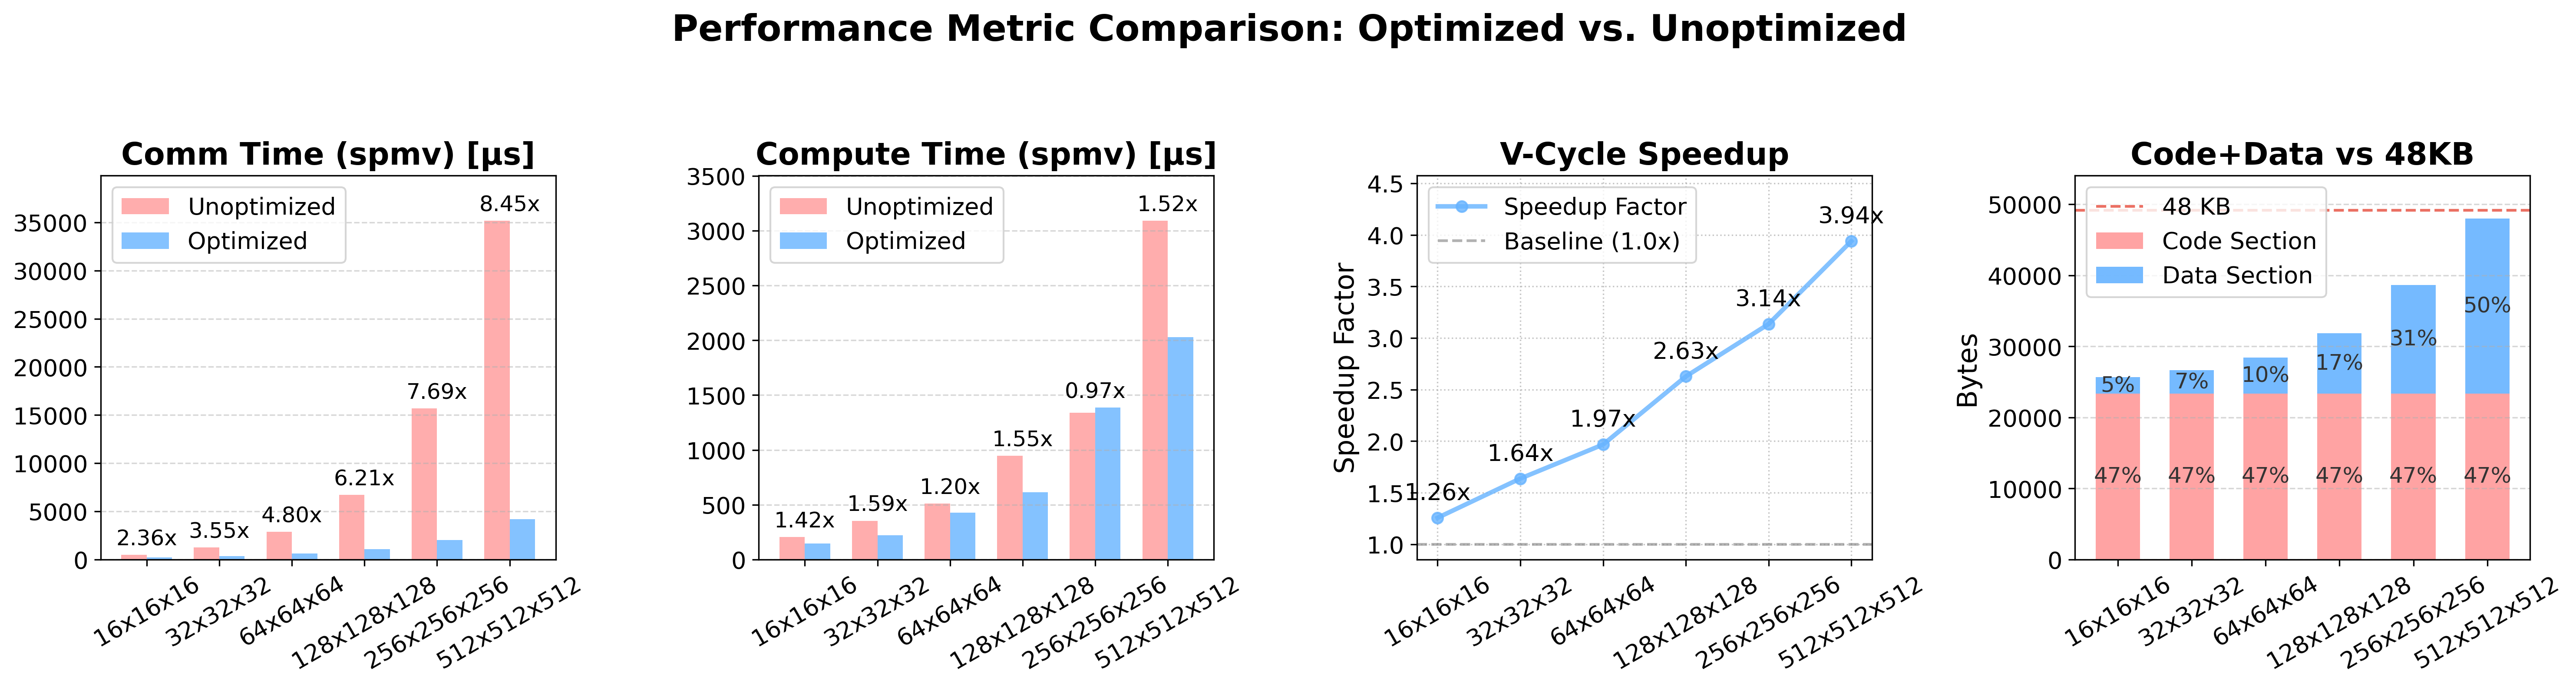
\includegraphics[width=\linewidth]{figures/metrics_comparison.png}
        \caption{Performance of HPGMG/Glow on Cerebras CS-3 and Nvidia GH200 using a $512^3$ grid with 9 multigrid levels, up to 100 iterations, a convergence tolerance of $1\times10^{-5}$, $4/4/6$ pre, post, and bottom smoothing steps, float32 precision, Jacobi relaxation $\omega=0.6667$, a 7-point stencil with $\alpha = -6.0$, $\beta = 1.0$, 16 channels, 256 block size, and a $762\times1172$ wafer fabric.}
        \label{fig:metrics-compare}
    \end{figure}

\subsection{Communication optimizations and memory constraints}
%\subsection*{E. Impact of optimizations and memory constraints}
    % let's start talking about metrics compare now.
    We further quantify the impact of our \textcolor{red}{You should have a name for this optimization in the Mapping section, and then you can refer to it by the name.} optimizations in Figure~\ref{fig:metrics-compare}. We show the gains due to optimizing the communication, our optimization shines as the number of inactive PEs start increasing, we see almost 8.45x speedup over unoptimized/inactive PE memory accessing implementation. This leads to a 3.94x speedup over the whole application shown in the bottom left corner. Compute time reduces since unnecessary computation on inactive PEs is also eliminated.
    
    The bottom-right panel of Figure 10 shows the breakdown of memory usage within a single processing element (PE), comparing the total available local memory against the size of the binary ELF image loaded on each PE. As shown, the code section alone occupies nearly 47\% of the available 48 KB SRAM and remains constant across multigrid levels. This is largely driven by aggressive function inlining performed by the backend LLVM compiler within the state-machine implementation, as well as the inclusion of stencil and collective-reduction library kernels. In contrast, the data section scales with problem size and the number of multigrid levels, reflecting the storage required for solution vectors, residuals, and intermediate buffers.Under the distributed superimposed mapping strategy adopted in this work, these memory constraints impose a practical limit on scalability. In particular, the fixed code footprint combined with per-level data storage restricts the ability to reduce per-PE data volume, effectively limiting experiments to weak scaling. Moreover, multigrid algorithms inherently require retaining data from finer levels during traversal, further constraining memory reuse under a distributed mapping.
    These observations highlight an important design trade-off for wafer-scale implementations for multilayered algorithms/applications. %, one such could be CNNs from the AI world. 
    Future approaches may benefit from hybrid mapping strategies that decouple computation and storage, such as assigning subsets of PEs primarily as memory resources while others focus on computation, or employing more dynamic coloring and routing schemes to reduce code replication and improve memory utilization across levels.

\section{Related Work}
%\paragraph{Stencils and GMG}
Historically, operations on large structured grids could easily be bound by capacity misses in cache, leading to a variety of studies on blocking and tiling optimizations to improve cache reuse on CPUs%[6, 8, 15, 19, 20, 27, 28].
%(an incomplete list might include
~\cite{Nguyen:2010:BOS:1884643.1884658,Zhou:2012,Yount:2016:YSK:3019129.3019133,Unat2016,Devito}. These techniques for multigrid have been successfully applied to finite-difference and finite-volume discretizations on shared-memory and distributed-memory systems.
As new supercomputer architectures evolve with higher peak multi-node performance, the growing gap between DRAM bandwidth and floating point operations (FLOPs) has focused research on increasing performance through data locality, particularly for bandwidth-bound computations.

Other efforts have introduced MG frameworks that could
efficiently exploit resources on GPU architectures. Examples
of recent multiphysics applications, where multigrid solvers
are key for elliptic equations, on structured or unstructured
grids include~\cite{Amrex,Anderson,Grete,mali}. Many of these efforts have been
focused on GPU acceleration and, to some extent performance
portability, since the focus is on different supercomputers with
different GPU vendors. However, because of the complexity
of multigrid solvers, it is an ongoing challenge to do detailed
performance analysis and explore optimization techniques
that exploit increasing GPU parallelism, GPU memory, and
network bandwidth.



%\paragraph{Stencils and Geometric Multigrid}
%~\cite{Nguyen:2010:BOS:1884643.1884658,Zhou:2012,Yount:2016:YSK:3019129.3019133,Unat2016,Devito}. 

\begin{comment}
\paragraph{Wafer-Scale Computing for Scientific Applications}
Several studies have ported scientific applications to wafer-scale architectures.  
(add links)  Purely stencil. Larger applications. Programming stacks.
\begin{itemize}
\item High-order stencil computations achieving near-perfect weak scaling~\cite{Sai,sai2}.
\item Matrix-free finite-volume solvers for subsurface flow.
\item Molecular dynamics simulations breaking timescale barriers.
\item Monte Carlo particle transport kernels with over 100× GPU speedup.
\item Communication collectives (Reduce/AllReduce) optimized for wafer-scale fabrics.
\end{itemize}
No published work has yet demonstrated GMG on Cerebras, making this study the first exploration.
\end{comment}
A growing body of work has demonstrated the effectiveness of wafer-scale systems for scientific computing. Early studies showed near-ideal weak scaling for high-order stencil computations and structured finite-difference operators on the WSE~\cite{scalable_25pt_stencil,Rocki,mathias,Sai,sai2}. Subsequent work extended these ideas to matrix-free finite-volume solvers for subsurface flow and seismic applications, highlighting the advantages of spatial data placement and explicit communication control~\cite{sai_fv_arxiv,Ltaief}. Larger application studies include molecular dynamics simulations that overcome traditional timescale barriers~\cite{perez_md_sc24,perez-journal} and Monte Carlo particle transport kernels achieving substantial speedups over GPU-based implementations~\cite{Tramm24,Yoshii26}. Communication-intensive primitives such as reductions and all-reductions have also been studied in isolation, with near-optimal collective implementations demonstrated on wafer-scale fabrics~\cite{luczynski_reduce}.

In parallel, several efforts have focused on improving programmability and compiler support for wafer-scale systems. These include DSL-based approaches for stencil computation~\cite{brown}, automated code generation for high-order stencils~\cite{sai_codegen_sc24}, and MLIR-based lowering pipelines targeting spatial dataflow architectures~\cite{stawinoga_mlir_stencils_wse}.
Spada is a programming language targeting spatial architectures that provides precise control over data placement, dataflow patterns, and asynchronous operations while abstracting architecture-specific low-level details~\cite{spada}.
While these works significantly advance kernel-level performance and developer productivity, they primarily target single-level stencil operators or application-specific kernels.%[spada is missing?]

To the best of our knowledge, no prior work has demonstrated a complete geometric multigrid solver mapped onto a wafer-scale architecture. GMG introduces additional challenges beyond single-level stencils, including multi-level data grids, coarse-grid solvers, and level-dependent communication patterns. This work represents the first end-to-end exploration of mapping a full GMG algorithm onto the Cerebras WSE-3 system, bridging the gap between prior stencil-centric studies and full multi-level scientific solvers.


\begin{comment}
I am commenting this out -- it breaks the flow, and it will be more work to do this well.
\textcolor{blue}{
Question: Is it worth to point what's happening in AI world for mapping layers on GPUs/WSE3?  This can connect AI layered mappings on Multigrid and show connection. Discard if not.
}
%* CNN mapping can be related work/any layered mapping application/algorithm.
* CNN mapping can be related work/any layered mapping application/algorithm.
* Distributed training of AI models and types of parallelism used - data parallel, model parallel, pipeline parallel, etc.
    https://towardsdatascience.com/distributed-parallel-training-data-parallelism-and-model-parallelism-ec2d234e3214/
\end{comment}

\begin{comment}
\section{Lessons Learned}
\begin{itemize}
\item Stencil-style, matrix-free kernels align best with CS-3; use them when structure allows.
\item AMG coarse operators generally require explicit sparse storage; use CSR/block-CSR within a PE and communicate only among nonzero-owning PEs.
\item Colors and custom routing schedules are indispensable to avoid contention and ensure determinism.
\item Developers must embrace matrix-free, fused-kernel approaches rather than porting sparse matrix libraries directly.
\item AMG represents the next step toward evaluating the architecture’s ability to handle irregular, graph-like scientific computations.
\end{itemize}
\textcolor{blue}{
\textbf{Lessons Learned:(dump, maybe not suitable here}
* Hardware fast, hard to program.
* Programming async and dataflow a new way of thinking compared to GPU(threadbased)
* Using AI for non-AI
* Tiled baseds hardwares and tiled based IR/Languges.
* Not right hardware for some type of applications.
* Memory is issue, need a shared + Distributed way to program this machine.
* Tooling debugger, profilers essential to have.
* shallower V-cycles are better matched to the wafer-scale architecture
\subsection*{Key Discussion/Take aways from results:}
\begin{itemize}
    \item We observe the GLOW is compute bound on finer levels and communication bound on coarser levels. 
    \item We observe having deep V cycles versus shallower V cycles yields significantly higher speedups with the cost of increased iterations to reach convergence.
    \item We think this application might not be a right fit for this architecture, we believe having a scaled out parallelism benefits from this machine rather than a distance dominating.
    \item We found having locality of data across PEs is the equivalent of data movement cost or cache equivalent costs in GPUs/CPUs. - Rewrite this
\end{itemize}

}
\end{comment}
\section{Conclusion}
We presented a mapping of GMG to WSE-3, achieving up to a $26\times$ speedup over a single node NVIDIA H200 GPU.  As this is, to our knowledge, the first mapping of GMG to WSE-2, this work exposes the challenges of achieving efficiency for layered algorithms, especially when memory size is so constrained.   
\textcolor{red}{What is the message from the experiment-- revisit some of the challenges,programming challenges.  In spite of these challenges, deterministic, high-bandwidth memory access times and local network lead to speedups over GPU.}
%that balances matrix-free efficiency with matrix-based generality. %Conceptual tables and figures clarify the programming model and architectural trade-offs. Future work will add empirical results, refine placement/routing for coarse levels, and explore portable abstractions for dataflow multigrid. AMG poses both opportunities and challenges on wafer-scale architectures. By reinterpreting its sparse, memory-bound kernels as streaming dataflow, we can leverage the WSE’s massive bandwidth and low-latency interconnect. Our analysis shows potential for compute-bound SpMV, efficient fine-level scaling, and bottlenecks at coarse levels. Future work will complete performance evaluation, explore adaptive coarsening layouts, and develop portable abstractions for AMG on dataflow hardware.
\begin{comment}
\section{Notes/thoughts/reviewer questions might be:}

\textbf{Q. Why is AMG not considered a good fit for WSE?}
We do not claim that AMG is inherently a poor fit for WSE, but rather that it remains unexplored. 
The complexity of the algorithm and the nature of sparsity in AMG present several implementation
and performance challenges on a wafer-scale engine (WSE):
\begin{itemize}
    \item \textbf{Sparsity representation:} AMG is well suited for unstructured problems, 
    where PDE discretizations\cite{b12} generate sparse matrices with highly irregular patterns. 
    Mapping such irregular sparsity efficiently onto WSE is non-trivial.
    
    \item \textbf{Communication bottlenecks:} Although the hardware fabric is low-latency, 
    AMG relies heavily on SpMV kernels. These can become communication-bound as both the 
    problem size and the PE grid size scale up, leading to potential bottlenecks across the wafer.
    
    \item \textbf{Routing limitations:} On WSE, communication links must pass through intermediate PEs. 
    Skipping over PEs that correspond to zero entries (as might be desirable in sparse operations) 
    is not feasible given hardware constraints.
    
    \item \textbf{Sparse matrix mapping challenge:} The problem essentially reduces to mapping a 
    sparse matrix across the wafer. While a local PE submatrix could use formats like BlockCSR 
    to reduce intra-PE operations, the irregular nature of input sparsity remains a major obstacle.
    
    \item \textbf{Irregular access and communication:} AMG is a general solver, but its irregular 
    communication and data access patterns conflict with the mesh-based organization of WSE. 
    
    \item \textbf{Open research direction:} Mapping irregular sparsity efficiently on WSE may 
    require revisiting older sparse data structures (previously deemed obsolete) or developing 
    entirely new ones tailored to large-scale, distributed wafer architectures.
\end{itemize}

\textbf{Matrix way partitioning strategy}
Instead of giving a processor a full row or column (which would require a lot of memory), checkerboard partitioning divides the sparse matrix into a grid of submatrices. A processor at location (i,j) in your PE grid is responsible for the submatrix Aij and the corresponding parts of the input vector xj and output vector yi.
Load Balancing: A simple uniform checkerboard might not work well for an irregular sparse matrix. To ensure even work distribution, you should use graph partitioning algorithms (like those from the Mondriaan or ParMETIS libraries) to cut the matrix into blocks that have roughly the same number of non-zero elements.
Memory Efficiency: By distributing the matrix non-zeros and vector elements across a million PEs, the memory requirement per PE becomes minimal. This is the only way to handle a large matrix on hardware with very little memory per processing unit.
2. Communication Strategy
The SpMV operation on a 2D grid involves two communication phases:
Column-wise Communication (Gather): Each processor (i,j) needs its part of the input vector xj. This means that all PEs in a given column of the processor grid must receive the same portion of the input vector. A broadcast or a collective gather operation along the processor columns is ideal for this. The PE that "owns" the j-th part of the vector x sends it to all PEs in its column.
Row-wise Communication (Accumulation): After each PE computes its partial result (Aijxj), these partial results must be summed up to form the final output vector y. This requires each PE (i,j) to send its partial result to all other PEs in its processor row. The final result yi is the sum of all partial results from the PEs in row i of the processor grid. This is typically done using a reduction or all-reduce operation along the processor rows.
\end{comment}
% \section*{References}
\nocite{*}
\bibliographystyle{IEEEtran}
\bibliography{refbibtex}

\section{Appendix}
* Show remaining problem size plots. 

\end{document}
